\chapter{Background and Preliminaries}
\label{chap:background}
\begin{figure}[h]
    \centering
    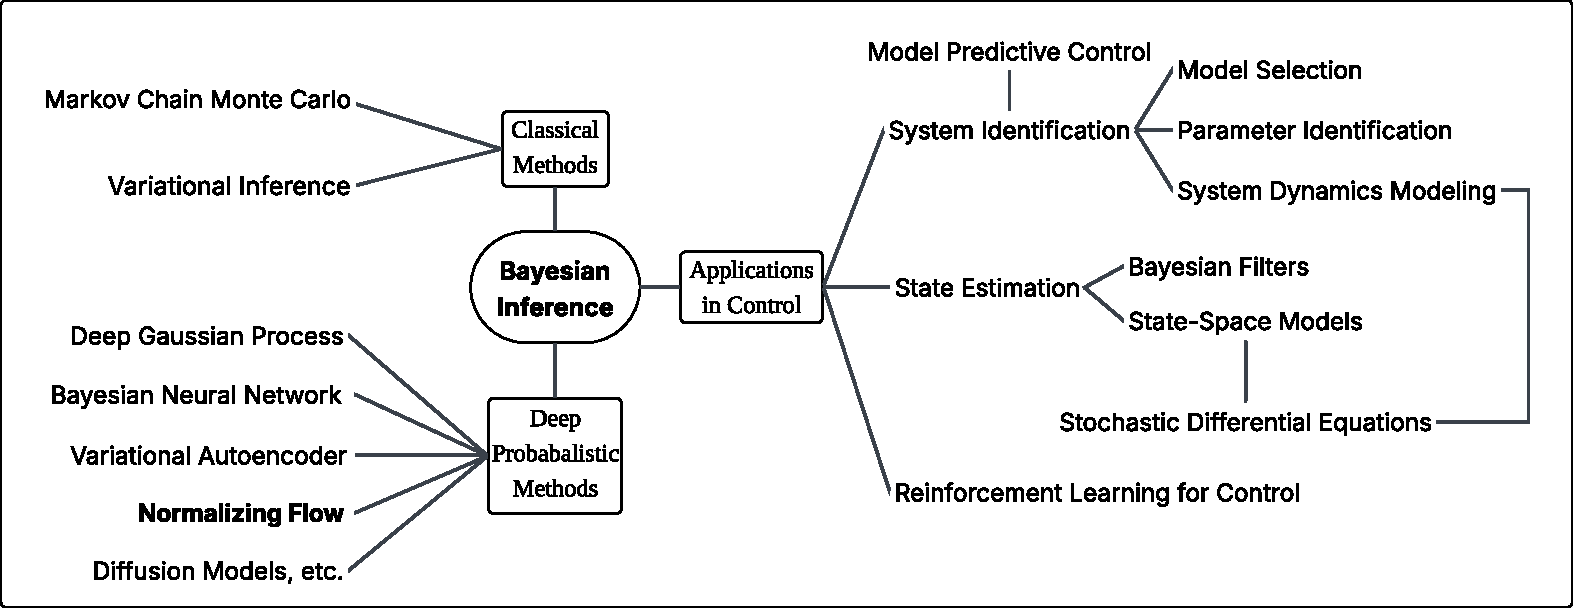
\includegraphics[width=\textwidth]{figures/Mindmap.pdf}
    \caption[Knowledge Map]{Conceptual map illustrating the integration of Bayesian inference with deep generative modeling and its applications in control engineering. The left side categorizes the modeling paradigms employed, moving from classical statistical methods to modern deep generative architectures. Notably, Normalizing Flows and Flow Matching are grouped together due to their shared theoretical foundation in continuous-time differential transformations and exact density estimation. On the right, the framework is mapped to core control tasks: system identification, state estimation, and optimal control. A dashed line connects Reinforcement Learning and Optimal Control, signifying the modern methodological convergence of these two disciplines where many data-driven learning methods can be viewed as an adaptive realization of classical optimal control theory.}
    \label{fig:knowledgemap}
\end{figure}
This section introduces the necessary foundational concepts and methodologies for understanding the rest of this work. Before the main content, we explain the unified notation used throughout this work. We first review classical Bayesian inference methods. Then we introduce deep probabilistic methods, including \acf{DGP}, \acf{BNN}, and \acf{VAE}. Next, we present the core methods of this work, \acfp{NF}, a powerful class of generative models for flexible density estimation. Finally, we bridge Bayesian inference to control methods, covering system identification, state estimation, and model predictive control. The overview for this chapter is shown in Figure~\ref{fig:knowledgemap}.

\section{Notations}

To maintain clarity throughout this document, we adopt the following notation:

\begin{table}[htbp!]
\centering
\renewcommand{\arraystretch}{1.5}
\begin{tabularx}{0.9\textwidth}{>{\bfseries}l X}
\toprule
Category & Description \\
\midrule
Basic Symbols &
Scalars: $x$; Vectors: $\boldsymbol{x}$; Matrices: $\boldsymbol{X}$; Sets: $\mathcal{D}$ \\
\midrule
Random Variables &
Multidimensional random variables: $\boldsymbol{x} = [x_1,\dots,x_D]^T$; Sample index: $\boldsymbol{x}^{(i)}$; Stochastic processes: $\mathit{X}(t)$ \\
\midrule
Time Series &
Time series of length $T$: $\boldsymbol{x}_{(1:T)}$; Time-dependent variables: $\boldsymbol{x}(t)$ or $x(t)$; Dimension index: $\boldsymbol{x}_i$ \\
\midrule
Variable Modifications &
Estimated: $\hat{\boldsymbol{x}}$; Transformed: $\tilde{\boldsymbol{x}}$; Time derivative: $\dot{\boldsymbol{x}}$ \\
\midrule
Probability and Statistics &
PDF: $p(\cdot)$; Joint PDF: $p(\cdot, \cdot)$; Conditional PDF: $p(\cdot |\cdot)$; Expectation: $\mathbb{E}_{p(x)}[f(x)]$; Covariance: $\operatorname{Cov}[\boldsymbol{x}, \boldsymbol{y}]$; Variance: $\operatorname{Var}[\boldsymbol{x}]$ \\
\midrule
Matrix Operations &
Identity: $\boldsymbol{I}$; Jacobian: $\boldsymbol{J}$; Determinant: $\det|\boldsymbol{J}|$; Trace: $\operatorname{Tr}(\boldsymbol{X})$; Transpose: $\boldsymbol{X}^\top$ \\
\bottomrule
\end{tabularx}
\caption{Notation Summary}
\label{tab:notation-summary}
\end{table}

\section{Bayesian Inference}
Bayesian inference gets its name from Bayes' rule, which is used to perform statistical inference over probability distributions.
This chapter draws on \textit{Bayesian Data Analysis} \citep{gelman2013bayesian}, \textit{Handbook of MCMC} \citep{Allen_2007}, and \textit{Variational Inference} \citep{Blei_2017}.

\subsection{Bayes' Rule}
Bayes' rule is derived from the chain rule of conditional probability. For target variables $\boldsymbol{\theta}$ and the corresponding observed data $\mathcal{D}$, the chain rule states that:
\begin{equation}
    p(\boldsymbol{\theta}, \mathcal{D}) = p(\boldsymbol{\theta}|\mathcal{D})p(\mathcal{D}) = p(\mathcal{D}|\boldsymbol{\theta})p(\boldsymbol{\theta}).
\end{equation}
Rearranging the terms gives Bayes' rule or Bayes' theorem:
\begin{equation}
\label{eq:bayes}
    p(\boldsymbol{\theta}|\mathcal{D})= \frac{p(\mathcal{D}|\boldsymbol{\theta})p(\boldsymbol{\theta})}{p(\mathcal{D})}.
\end{equation}
In Bayes' theorem, $p(\boldsymbol{\theta})$ is the initial distribution of the variables before any data samples are considered, which is called the \textit{prior distribution}. $p(\boldsymbol{\theta}|\mathcal{D})$ is the posterior distribution of the target variables after being updated by the observed data. $p(\mathcal{D}|\boldsymbol{\theta})$ is the likelihood of expected data given the setting of parameters $\boldsymbol{\theta}$. $p(\mathcal{D})$ is called the \textit{marginal likelihood} or \textit{evidence} of expected data across all possible variable settings:
\begin{subequations}
    \begin{align}
    p(\mathcal{D}) &= \Sigma_{\boldsymbol{\theta}'}p(D|\boldsymbol{\theta}')p(\boldsymbol{\theta}')\Delta \boldsymbol{\theta}',\\
    p(\mathcal{D}) &= \int p(D|\boldsymbol{\theta}')p(\boldsymbol{\theta}')d\boldsymbol{\theta}'.
    \end{align}
\end{subequations}
In practice, it is often treated as a normalizing constant and ignored. The unnormalized posterior is then given by:
\begin{equation}
    p_u(\boldsymbol{\theta}|\mathcal{D}) \propto p(\mathcal{D}|\boldsymbol{\theta})p(\boldsymbol{\theta}).            
\end{equation}

Normally, the posterior distribution does not have a closed-form expression. Instead, we approximate it using numerical methods. Computational algorithms that rely on repeated random sampling to obtain numerical results are referred to as "Monte Carlo" methods. Monte Carlo methods provide ways to approximate the posterior distribution by expectations:
\begin{equation}
    E=\mathbb{E}_{p(\boldsymbol{\theta}|\mathcal{D})}[f(\boldsymbol{\theta})] = \int f(\boldsymbol{\theta}) p(\boldsymbol{\theta}|\mathcal{D}) d\boldsymbol{\theta},
\end{equation}
where $f(\boldsymbol{\theta})$ is any function of interest, for example, $f(\boldsymbol{\theta})=\boldsymbol{\theta}$. In the simplest case, we can approximate it using standard numerical techniques such as a Riemann sum over a discrete grid of points:
\begin{equation}
    E \approx \Sigma_{\boldsymbol{\theta}'} f(\boldsymbol{\theta}') \Delta \boldsymbol{\theta}'.
\end{equation}
However, this approach is only feasible for low-dimensional $\boldsymbol{\theta}$ due to the curse of dimensionality. Moreover, for complex distributions, the discretization is highly inefficient. Therefore, for high-dimensional parameters and complex distributions, we often resort to sampling-based or optimization-based methods to approximate the posterior distribution, which will be discussed in the following sections.

\subsection{Markov Chain Monte Carlo}
The "Markov Chain" aspect indicates that these algorithms generate a sequence of samples in which each sample depends only on the previous one. In contrast to the basic Monte Carlo methods, \acf{MCMC} methods produce auto-correlated samples, so that each new sample adds less new information than an independent draw would. Different sequence-update algorithms lead to different \ac{MCMC} methods. The goal of \ac{MCMC} is to construct a Markov chain that has the desired posterior distribution as its \textit{equilibrium} distribution. After running the chain for a sufficient number of iterations, the samples generated from the chain can be treated as samples from the target posterior distribution. 

This concept is analogous to the steady-state behavior of a dynamical system. Typically, a dynamical system undergoes a transient phase before settling into an equilibrium where the states remain constant. In \ac{MCMC}, while the variables continue to move, their probability distribution reaches a steady state. If we interpret the probability density as the energy landscape of a physical system, equilibrium is reached when the system has settled into a stable statistical configuration. At this point, although individual samples continue to transition between different regions of the parameter space, the net movement between these regions is zero. This balance ensures that the density of samples remains constant over time, allowing the chain to accurately represent the invariant target posterior distribution.

\subsubsection{Metropolis-Hastings Algorithm}
\begin{table}[htbp]
    \centering
    \small
    \begin{tabular}{>{\raggedright\arraybackslash}p{0.55\textwidth} | >{\raggedright\arraybackslash}p{0.43\textwidth}}
    \toprule
    \textbf{MH Algorithm (Random Walk) } & \textbf{Autonomous Rover Mapping} \\ 
    \midrule
    \textbf{1. Initialization} & \textbf{1. Power-On \& Config} \\
    Set starting point $\boldsymbol{\theta}_{(0)}$.  & The rover starts at GPS coordinate $\boldsymbol{\theta}_{(0)}$.\\Define proposal $q(\boldsymbol{\theta}'|\boldsymbol{\theta})$, which is usually a Gaussian $\mathcal{N}(\boldsymbol{\theta}, \sigma^2)$. & 
    Set the Jogging Logic ($q$): a random-walk jump distance based on motor constraints. \\
    \midrule
    \textbf{2. Iteration Loop} (for each $i$): & \textbf{2. Navigation Duty Cycle}: \\
    \midrule
    \textit{(a) Propose a new state:} & \textit{(a) Candidate Path Planning:} \\
    Generate a candidate $\boldsymbol{\theta}'_{(i)}$ using the proposal distribution $q(\boldsymbol{\theta}'_{(i)}|\boldsymbol{\theta}_{(i-1)})$. & 
    A phantom coordinate $\boldsymbol{\theta}'_{(i)}$ nearby is calculated. This is a potential move, but the actuators are not yet engaged. \\
    \midrule
    \textit{(b) Calculate Transition Probability $T(\boldsymbol{\theta}'_{(i)}|\boldsymbol{\theta}_{(i-1)})$:} & \textit{(b) Sensor Evaluation based on Data $\mathcal{D}$:} \\
    \begin{minipage}{0.48\textwidth}
        \begin{equation}
        \label{eq:mh_transition}
            T(\boldsymbol{\theta}'_{(i)}|\boldsymbol{\theta}_{(i-1)}) = \min\!\left(
            \begin{array}{l}
            1,\\[2pt]
            \dfrac{p(\boldsymbol{\theta}'_{(i)}\mid\mathcal{D})\,q(\boldsymbol{\theta}_{(i-1)}\mid\boldsymbol{\theta}'_{(i)})}{p(\boldsymbol{\theta}_{(i-1)}\mid\mathcal{D})\,q(\boldsymbol{\theta}'_{(i)}\mid\boldsymbol{\theta}_{(i-1)})}
            \end{array}
            \right)
        \end{equation}
    \end{minipage}
    &
    The rover asks: "Based on our sensor history ($\mathcal{D}$), is the ice likely denser at the phantom spot $\boldsymbol{\theta}'$ than my current spot $\boldsymbol{\theta}$?" It also checks for mechanical bias in $q$. \\
    \midrule
    \textit{(c) Update via Accept/Reject:} & \textit{(c) Actuator Actuation:} \\
    \begin{minipage}{0.48\textwidth}
        \begin{equation}
        \label{eq:mh_update}
        \boldsymbol{\theta}_{(i)} =
        \begin{cases} \boldsymbol{\theta}'_{(i)}, & \text{if } u < T(\boldsymbol{\theta}'_{(i)}|\boldsymbol{\theta}_{(i-1)}) \\ \boldsymbol{\theta}_{(i-1)}, & \text{otherwise} 
        \end{cases}
        \end{equation}
    \end{minipage}
    & 
    If the spot is "better," the motors drive there. If "worse," it rolls a die: it might still move there to explore, or stay put and record the current spot again. \\
    \midrule
    \textbf{3. Accumulation} & \textbf{3. Mission Duration} \\
    Run the chain for more than $N_{\mathrm{burn}}$ iterations. The first $N_{\mathrm{burn}}$ samples are treated as burn-in, after which the chain is assumed to have reached its stationary distribution. The retained samples are $\{\boldsymbol{\theta}_{(N_{\mathrm{burn}}+1)}, \ldots, \boldsymbol{\theta}_{(N_{\mathrm{burn}}+B)}\}$. & 
    The rover first drives long enough to leave its arbitrary starting region and reach a representative exploration pattern. Only after this warm-up period does it write the subsequent $(x,y)$ coordinates into the mission logbook. \\
    \midrule
    \textbf{4. Estimator} & \textbf{4. Resource Density Map} \\
    \[p(\boldsymbol{\theta}| \mathcal{D}) \approx \frac{1}{B} \sum_{b=1}^{B} \delta_{(N_{\mathrm{burn}}+b)}(\boldsymbol{\theta})\] 
    $\delta_{(N_{\mathrm{burn}}+b)}(\boldsymbol{\theta})$ denotes a Dirac delta centered at the retained sample $\boldsymbol{\theta}_{(N_{\mathrm{burn}}+b)}$.
    & 
    Download the log and plot the coordinates. The resulting point cloud density shows the ice distribution $p(\boldsymbol{\theta}|\mathcal{D})$ across the crater. \\
    \bottomrule
    \end{tabular}
    \caption[Alignment between MH Algorithm and Autonomous Rover Mapping]{Alignment between the Metropolis-Hastings (MH) algorithm and an autonomous rover mapping.}
    \label{tab:comp_mh}
\end{table}
The \ac{MH} algorithm, which is named after Metropolis \citeyearpar{Metropolis} and Hastings \citeyearpar{Hastings}, is a widely used \ac{MCMC} method. To understand its logic, consider the "Autonomous Rover Mapping" analogy: Imagine an autonomous rover equipped with a noisy sensor is deployed into a dark and unmapped crater. Its task is to create a high-resolution density map of water-ice concentrations across the crater floor. It doesn't have a satellite map; it only knows the signal strength of ice at its current coordinates using a neutron spectrometer. It cannot teleport and thus has to move from point to point in order to take readings. The density map is essentially a confidence map of where the ice is located $(\boldsymbol{\theta})$ given the sensor observations $(\mathcal{D})$. An alignment between the MH algorithm and its analogy is shown in Table~\ref{tab:comp_mh}.

Although this procedure allows flexible approximation of complex posterior distributions, it suffers from a slow convergence rate because of its random exploration strategy. Thus, gradient-based \ac{MCMC} methods are proposed to incorporate the structure of the target density, leading to faster sampling.

\subsubsection{Metropolis-Adjusted Langevin Algorithm}\label{sec:MALA}
The \ac{MALA} \citep{besag2004markov} combines the \ac{MH} algorithm with Langevin diffusion, whose stationary distribution is the target density. In this framework, 
the rover no longer jumps blindly; instead, it uses its onboard sensors to detect the local slope of the resource distribution. Its movement is then governed by a first-order control law consisting of two parts: a deterministic drift that pushes the rover uphill toward higher density, and a stochastic diffusion (Gaussian noise) that ensures the rover continues to explore rather than getting stuck at a single peak.

In general, for a stochastic process $\mathit{\Theta}(t)$ for variables $\boldsymbol{\theta}$, the Langevin diffusion is described by the following \ac{SDE}:
\begin{equation}
    d\mathit{\Theta}(t)=\nabla \log p(\mathit{\Theta}(t))dt + \sqrt{2} d\mathit{W}(t),
\end{equation}
where $\mathit{W}(t)$ denotes a standard Wiener process \citep{gabbiani2010mathematics}. The Wiener process is a continuous-time stochastic process with independent, normally distributed increments, which can be interpreted as Brownian motion. It has the following properties:
\begin{enumerate}
    \item [(1)] $\mathit{W}(0)=\boldsymbol{0}$;
    \item [(2)] for $t > s \geq 0 $, $\mathit{W}(t)-\mathit{W}(s)\sim\sqrt{t-s}\;\mathcal{N}(\boldsymbol{0}, \boldsymbol{I})$;
    \item [(3)] for $t_1>s_1\geq 0$, and $t_2>s_2\geq 0$, $\mathit{W}(t_1)-\mathit{W}(s_1)$ and $\mathit{W}(t_2)-\mathit{W}(s_2)$ are independent. 
\end{enumerate}         

\begin{figure}[htbp]
    \begin{minipage}{0.65\textwidth}
        \centering
        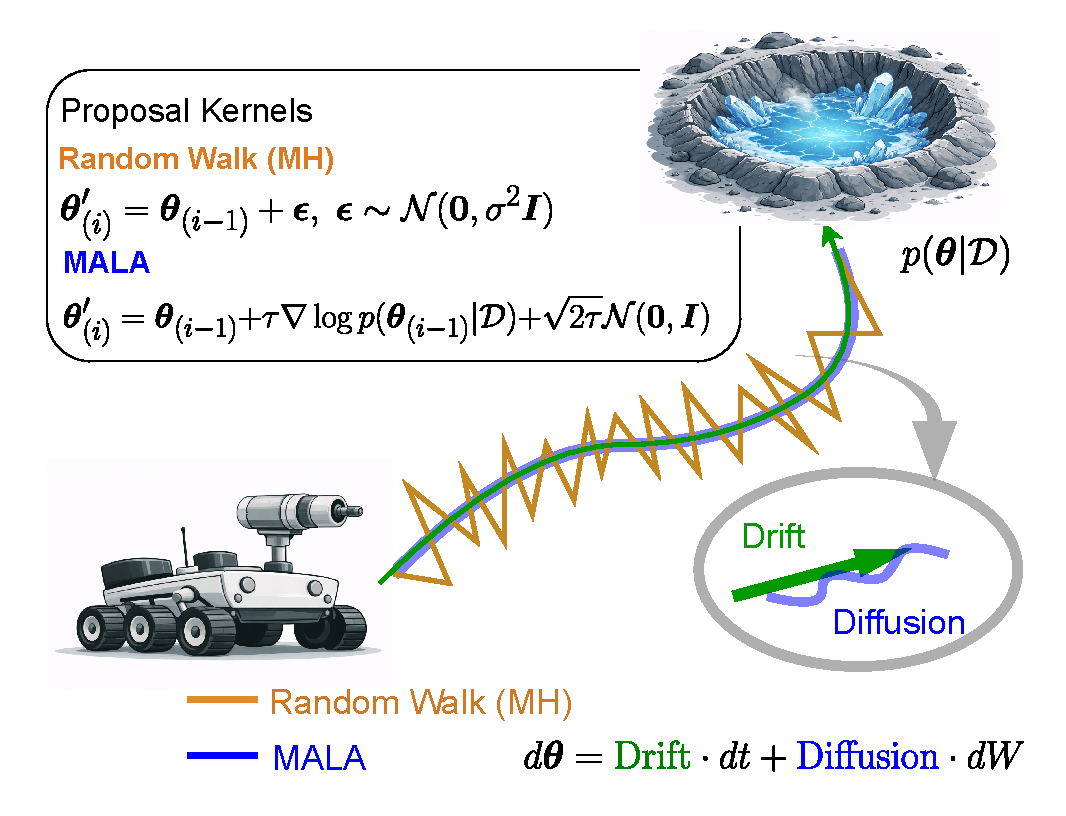
\includegraphics[width=0.9\textwidth]{figures/mh_mala.pdf}
    \end{minipage}
    \begin{minipage}{0.32\textwidth}
        \caption[MH MALA Comparison]{An illustration of \ac{MH} algorithm and \ac{MALA} using the autonomous rover as a conceptual sampler. The crater representing $p(\boldsymbol{\theta|\mathcal{D}})$ serves as the objective landscape where the sampler aims to concentrate its states. The Random Walk (MH) is shown as the jagged orange path, while the \ac{MALA} is represented by a smoother green path (drift) along with a blue band (diffusion).}
        \label{fig:mh_mala}
    \end{minipage}
\end{figure}

A comparison between the \ac{MH} algorithm and \ac{MALA} is illustrated in Figure~\ref{fig:mh_mala}. The \ac{MALA} uses the first-order Euler-Maruyama discretization of the \ac{SDE}, resulting in the following proposal distribution:
\begin{equation}
    \label{eq:langevin}
    \mathit{\Theta}(t) = \mathit{\Theta}(i-1) + \tau \nabla \log p(\mathit{\Theta}(i-1)) + \sqrt{2\tau}\; \mathcal{N}(\boldsymbol{0}, \boldsymbol{I}),
\end{equation}
where $\tau$ is a step size parameter.
Because of the discretization, convergence to the target density is no longer guaranteed. Therefore, the \ac{MH} algorithm is applied to correct the bias introduced by the discretization. 
For each iteration $i$, the \ac{MALA} updates the state as follows (corresponding to the iteration part in Table~\ref{tab:comp_mh}):
\begin{enumerate}[noitemsep,topsep=2pt]
    \item[(a)] \textbf{Guidance with Gradient:} Unlike the uninformed \ac{MH}, which only considers the current position, \ac{MALA} first computes the gradient of the log-posterior: $\nabla \log p(\boldsymbol{\theta}_{(i-1)}|\mathcal{D})$. This determines the drift direction toward regions of higher probability.
    \item[(b)] \textbf{Informed Proposal:} Propose a new state $\boldsymbol{\theta}'_{(i)}$ using the Langevin dynamics (\ref{eq:langevin}): $\boldsymbol{\theta}'_{(i)} = \boldsymbol{\theta}_{(i-1)} + \tau \nabla \log p(\boldsymbol{\theta}_{(i-1)}) + \sqrt{2\tau}\; \mathcal{N}(\boldsymbol{0}, \boldsymbol{I})$.
    \item[(c)] \textbf{Transition Probability:} Calculate the transition probability according to Equation~(\ref{eq:mh_transition}). Specifically, the proposal distribution is derived from the Langevin dynamics:
    \begin{equation}
        q(\boldsymbol{\theta}'_{(i)}|\boldsymbol{\theta}_{(i-1)})\propto \exp(-\frac{1}{4\tau}\left\|\boldsymbol{\theta}'_{(i)}-\boldsymbol{\theta}_{(i-1)}-\tau\nabla\log p(\boldsymbol{\theta}_{(i-1)}|\mathcal{D})\right\|^2_2).
    \end{equation}
    \item[(d)] \textbf{Correction (Accept/Reject):} Using the same mechanism as MH, a uniform random number $u \sim U(0,1)$ is generated. Then, the state $\boldsymbol{\theta}_{(i)}$ is updated by the accepting ratio according to Equation~(\ref{eq:mh_update}). 
\end{enumerate}

Compared to the \ac{MH}, \ac{MALA} converges faster and scales better in higher dimensions, at the cost of requiring gradients and tuning. As a more advanced \ac{MCMC} method, \acf{HMC} \citep{duane1987hybrid} further improves sampling efficiency by simulating the whole sampling trajectory as Hamiltonian dynamics. 

\subsection{Variational Inference}
Unlike \ac{MCMC}, \acf{VI} \citep{Jordan1998, Wainwright2008} is an optimization-based method that approximates the target posterior distribution $p(\boldsymbol{\theta}|\mathcal{D})$ with a simpler, parameterized distribution $q_{\boldsymbol{\phi}}(\boldsymbol{\theta})$, where $\boldsymbol{\phi}$ denotes the variational factors. The goal of \ac{VI} is to find the optimal variational factors $\boldsymbol{\phi}^*$ that minimize the distance between the approximate distribution and the true posterior. The distance is normally measured by the \ac{KL}-divergence \citep{kl1951}, which is defined as:
\begin{equation}
    D_{\text{KL}}(q(z)||p(z)) = \mathbb{E}_{q(z)}[\log \frac{q(z)}{p(z)}] = \int q(z)\log \frac{q(z)}{p(z)}dz.
\end{equation}
Thus, the optimization problem of \ac{VI} can be formulated as:
\begin{equation}
    \boldsymbol{\phi}^* = \arg\min_{\boldsymbol{\phi}} D_{\text{KL}} (q_{\boldsymbol{\phi}}(\boldsymbol{\theta}) || p(\boldsymbol{\theta}|\mathcal{D})).
\end{equation}
Substituting Bayes' rule (\ref{eq:bayes}) into \ac{KL}-divergence, we have:
\begin{equation}
    D_{\text{KL}} (q_{\boldsymbol{\phi}}(\boldsymbol{\theta}) || p(\boldsymbol{\theta}|\mathcal{D})) = D_{\text{KL}} (q_{\boldsymbol{\phi}}(\boldsymbol{\theta}) \,||\, \textcolor{blue}{\frac{p(\mathcal{D}|\boldsymbol{\theta})p(\boldsymbol{\theta})}{p(\mathcal{D})}}).
\end{equation}
The marginal likelihood $p(\mathcal{D})$ is usually intractable, as it involves integrating over all possible parameter settings. Therefore, the divergence cannot be computed directly.

Expanding the above equation with the definition of \ac{KL}-divergence, we have:
\begin{multline}
    D_{\text{KL}}(q_{\boldsymbol{\phi}}(\boldsymbol{\theta}) || p(\boldsymbol{\theta}|\mathcal{D})) = \textcolor{blue}{\mathbb{E}_{q_{\boldsymbol{\phi}}(\boldsymbol{\theta})}[\log q_{\boldsymbol{\phi}}(\boldsymbol{\theta}) - \log p(\mathcal{D}|\boldsymbol{\theta}) - \log p(\boldsymbol{\theta}) + \log p(\mathcal{D})]}\\
    = \mathbb{E}_{q_{\boldsymbol{\phi}}(\boldsymbol{\theta})}\log q_{\boldsymbol{\phi}}(\boldsymbol{\theta})-\mathbb{E}_{q_{\boldsymbol{\phi}}(\boldsymbol{\theta})}\log p(\mathcal{D}|\boldsymbol{\theta})-\mathbb{E}_{q_{\boldsymbol{\phi}}(\boldsymbol{\theta})}\log p(\boldsymbol{\theta}) + \textcolor{blue}{\mathbb{E}_{q_{\boldsymbol{\phi}}(\boldsymbol{\theta})}\log p(\mathcal{D})}.
\end{multline}
Since $p(\mathcal{D})$ is independent of the variational factors $\boldsymbol{\phi}$, the last term is reduced to $\textcolor{blue}{\log p(\mathcal{D})}$.
Combining the terms $p(\mathcal{D}|\boldsymbol{\theta})p(\boldsymbol{\theta})=\textcolor{ForestGreen}{p(\boldsymbol{\theta}, \mathcal{D})}$ gives
\begin{equation}
    \label{eq:vi_kl1}
    D_{\text{KL}}(q_{\boldsymbol{\phi}}(\boldsymbol{\theta}) || p(\boldsymbol{\theta}|\mathcal{D})) = \mathbb{E}_{q_{\boldsymbol{\phi}}(\boldsymbol{\theta})}\log q_{\boldsymbol{\phi}}(\boldsymbol{\theta})-\mathbb{E}_{q_{\boldsymbol{\phi}}(\boldsymbol{\theta})}\log \textcolor{ForestGreen}{p(\boldsymbol{\theta}, \mathcal{D})} + \log p(\mathcal{D})
\end{equation}
Or combining the terms $q_{\boldsymbol{\phi}}(\boldsymbol{\theta})$ and $p(\boldsymbol{\theta})$ via \ac{KL}-divergence gives:
\begin{equation}
    \label{eq:vi_kl2}
    D_{\text{KL}}(q_{\boldsymbol{\phi}}(\boldsymbol{\theta}) || p(\boldsymbol{\theta}|\mathcal{D}))=\textcolor{Sepia}{D_{\text{KL}}(q_{\boldsymbol{\phi}}(\boldsymbol{\theta})||p(\boldsymbol{\theta}))} - \textcolor{Sepia}{\mathbb{E}_{q_{\boldsymbol{\phi}}(\boldsymbol{\theta})}\log p(\mathcal{D}|\boldsymbol{\theta})} + \log p(\mathcal{D})
\end{equation}
Rearranging the terms in Equation~(\ref{eq:vi_kl1}) gives:
\begin{equation}
    \log p(\mathcal{D}) = \textcolor{blue}{D_{\text{KL}}(q_{\boldsymbol{\phi}}(\boldsymbol{\theta}) || p(\boldsymbol{\theta}|\mathcal{D}))}+\mathbb{E}_{q_{\boldsymbol{\phi}}(\boldsymbol{\theta})}\log p(\boldsymbol{\theta}, \mathcal{D})-\mathbb{E}_{q_{\boldsymbol{\phi}}(\boldsymbol{\theta})}\log q_{\boldsymbol{\phi}}(\boldsymbol{\theta}).
\end{equation} 
Since the \ac{KL}-divergence is always non-negative, we have:
\begin{mdframed}[nobreak=true]
    \begin{equation}
        \label{eq:elbo1}
        \log p(\mathcal{D}) \geq \textcolor{ForestGreen}{\mathbb{E}_{q_{\boldsymbol{\phi}}(\boldsymbol{\theta})}\log p(\boldsymbol{\theta}, \mathcal{D})-\mathbb{E}_{q_{\boldsymbol{\phi}}(\boldsymbol{\theta})}\log q_{\boldsymbol{\phi}}(\boldsymbol{\theta})}.
    \end{equation}
\end{mdframed}
Because of this inequality, the right-hand side is called the \acf{ELBO}, also known as the variational lower bound. Another way to formulate the \ac{ELBO} using Equation~(\ref{eq:vi_kl2}) is:
\begin{mdframed}[nobreak=true]
    \begin{equation}
        \label{eq:elbo2}
        \text{ELBO} = \textcolor{Sepia}{\mathbb{E}_{q_{\boldsymbol{\phi}}(\boldsymbol{\theta})}\log p(\mathcal{D}|\boldsymbol{\theta})} - \textcolor{Sepia}{D_{\text{KL}}(q_{\boldsymbol{\phi}}(\boldsymbol{\theta})||p(\boldsymbol{\theta}))}. 
    \end{equation}
\end{mdframed}
Then, minimizing the \ac{KL}-divergence is equivalent to maximizing the \ac{ELBO} (\ref{eq:elbo1}), leading to the equivalent optimization problem:
\begin{equation}
    \label{eq:vi_opt}
    \boldsymbol{\phi}^* = \arg\max_{\boldsymbol{\phi}} \text{ELBO} = \arg\min_{\boldsymbol{\phi}}[\mathbb{E}_{q_{\boldsymbol{\phi}}(\boldsymbol{\theta})}\log q_{\boldsymbol{\phi}}(\boldsymbol{\theta})-\mathbb{E}_{q_{\boldsymbol{\phi}}(\boldsymbol{\theta})}\log p(\boldsymbol{\theta}, \mathcal{D})].
\end{equation}

To complete the optimization, we need to choose a suitable family of variational distributions $q_{\boldsymbol{\phi}}(\boldsymbol{\theta})$. A common choice is the mean-field family \citep{bishop2006}, which assumes that the variables $\boldsymbol{\theta}$ are mutually independent and each governed by a distinct factor under $q$:
\begin{equation}
    q_{\boldsymbol{\phi}}(\boldsymbol{\theta}) = \Pi_{i} q_{\phi_i}(\theta_i),
\end{equation}
where each factor $\phi_i$ governs a variable $\theta_i$. Then, the \ac{ELBO} (\ref{eq:elbo1}) is iteratively optimized by updating each factor while holding the others fixed. The solution of the optimal distribution $q_{\phi_i}(\theta_i)$ is proportional to the exponential expected log of the complete condition:
\begin{equation}
    \log q_{\phi_i}^*(\theta_i) \propto \mathbb{E}_{\Pi_{j\neq i}q_{\phi_i}(\theta_i)}[\log p(\theta_i|\boldsymbol{\theta}_{j\neq i}, \mathcal{D})],
\end{equation}
where the expectation is taken with respect to the distributions of all other groups $j \neq i$. This algorithm is called \ac{CAVI} \citep{bishop2006}. 

The assumption of the mean-field \ac{VI} simplifies the optimization problem, and thus makes it scalable for high-dimensional variables and also enables parallelizable computation. However, it may also limit the expressiveness of the variational distribution, especially when the posterior correlations are crucial, leading to suboptimal approximations of the true posterior. In summary, \ac{VI} is generally faster than \ac{MCMC} and scales better to large datasets, but it may provide less accurate approximations of the posterior distribution \citep{Blei_2017}. 

\section{Deep Probabilistic Methods}
\label{sec:introduction:background:deep_probabilistic_methods}
Although classical methods such as \ac{MCMC} and \ac{VI} provide general solutions for Bayesian inference, they are limited by their "approximation-per-point" behavior. Deep probabilistic methods, in contrast, enable amortized Bayesian inference and unlock both high expressiveness and scalability to large datasets. In the following section, we briefly review three prominent deep probabilistic methods: the Deep Gaussian Process, the Bayesian Neural Network, and the Variational Autoencoder. The former two methods are direct extensions of classical Bayesian inference with deep architectures, while the last one is a fundamental deep generative model that leverages variational inference.

\subsection{Deep Gaussian Process}
A Gaussian process can be interpreted as an infinite-dimensional Gaussian distribution. It is fully specified by a mean function $m(\cdot)$ and a covariance (kernel) function $k(\cdot, \cdot)$. For simplicity, we consider a single-variable case where the variable is $x$ and the corresponding Gaussian process is $\mathit{X}(t)$. We collect $M$ observations at discrete input points $\boldsymbol{x} = [x_1, \dots, x_M]^\top$, the associated random variables follow a multivariate normal distribution:
\begin{equation}
    \begin{bmatrix} \mathit{X}(t_1) \\ \vdots \\ \mathit{X}(t_M) \end{bmatrix} \sim \mathcal{N} \left( \boldsymbol{\mu}=\begin{bmatrix} \mu(t_1) \\ \vdots \\ \mu(t_M) \end{bmatrix}, \boldsymbol{K}=\begin{bmatrix} k(t_1, t_1) & \dots & k(t_1, t_M) \\ \vdots & \ddots & \vdots \\ k(t_M, t_1) & \dots & k(t_M, t_M) \end{bmatrix} \right).
\end{equation}
Note that the time here is not really temporal but indicates the coordinates of variables in the parameter domain. For example, the $t_i$-th observation in the dataset is $x_i$. Thus, in the following, we call $t_i$ an index, instead of a time point. Using a Gaussian process to infer variables from observed data based on prior distributions leads to \ac{GPR} \citep{Rasmussen_Williams_2008}. In comparison to \ac{MCMC}, \ac{GPR} aims to directly approximate the target distribution function with a Gaussian-based surrogate model instead of sampling them iteratively.

\subsubsection{Gaussian Process Regression}
We assume that we observe noisy measurements $\boldsymbol{y} = [y_1, \dots, y_M]^\top$ at inputs $\boldsymbol{x}$. The observation model relates the latent function $f(\cdot)$ to the observations via additive Gaussian noise:
\begin{equation}\label{eq:simgp}
y_i = f(x_i) + \epsilon_i, \qquad \epsilon_i \sim \mathcal{N}(0,\sigma_\epsilon^2).
\end{equation}
The likelihood $p(y_i|f(x_i))$ is thus given by:
\begin{equation}
    p(y_i|f(x_i))=\mathcal{N}(y_i|f(x_i), \sigma_{\epsilon}^2).
\end{equation}

The prior distribution over functions $f(\cdot)$ is assumed to be a zero-mean Gaussian process:
\begin{equation}
    f(\cdot)\sim\mathcal{GP}(0, k(\cdot, \cdot)).
\end{equation}
The kernel function $k(\cdot,\cdot)$ is usually chosen as the \ac{SE} kernel, also known as the \ac{RBF}, defined as:
\begin{equation}
    k(x_i, x_j) = \sigma_{SE}^2\exp(-\frac{1}{2\ell^2}\left\| x_i - x_j\right\|^2),
\end{equation}
where $\sigma_{SE}$ and $\ell$ are vertical and horizontal scale parameters, which control the vertical span and smoothness of the function, respectively.

To obtain the optimal regression performance, the hyperparameters $\varphi = \{ \sigma_{SE}, \ell, \sigma_{\epsilon} \}$ must be optimized. In \ac{GPR}, this is achieved by maximizing the log marginal likelihood. By integrating out the latent function values $f$, the marginal distribution of the data $\boldsymbol{y}$ depends only on the inputs $\boldsymbol{x}$ and hyperparameters $\varphi$:
\begin{equation}
    p(\boldsymbol{y} | \boldsymbol{x}, \varphi) = \mathcal{N}(\boldsymbol{y} | \boldsymbol{0}, \boldsymbol{K} + \sigma_{\epsilon}^2 \boldsymbol{I}).
\end{equation}
The optimization objective $\mathcal{J}(\varphi)$ is the logarithm of this marginal likelihood:
\begin{equation}
    \mathcal{J}(\varphi) = \log p(\boldsymbol{y} | \boldsymbol{x}, \varphi) = -\underbrace{\frac{1}{2} \boldsymbol{y}^\top (\boldsymbol{K} + \sigma_{\epsilon}^2 \boldsymbol{I})^{-1} \boldsymbol{y}}_{\text{Data Fit}} - \underbrace{\frac{1}{2} \log | \boldsymbol{K} + \sigma_{\epsilon}^2 \boldsymbol{I} |}_{\text{Complexity Penalty}} - \frac{M}{2} \log 2\pi.
\end{equation}
The optimal hyperparameters $\hat{\varphi}$ are found by maximizing this function, typically using gradient-based optimizers.

The \ac{GPR} is widely used for regression tasks owing to its non-parametric nature and its capacity to quantify uncertainty. However, its computational complexity scales cubically with the number of training points, i.e., $\mathcal{O}(D^3)$ for a $D$-dimensional input. Additionally, calculating Gaussian processes requires storing the entire training dataset, incurring a memory cost of $\mathcal{O}(M^2)$, which grows quadratically with the dataset size $M$. These limitations hinder its scalability to high-dimensional inputs and large datasets. In addition, the expressiveness of \ac{GPR} is constrained by the choice of kernel function and its incapacity to perform hierarchical feature extraction.

\subsubsection{Parameter Identification using GPR}
\begin{table}[ht]
    \centering
    \small
    \renewcommand{\arraystretch}{1.5}
    \begin{tabularx}{\textwidth}{@{} p{0.18\textwidth} >{\hsize=0.8\hsize}X >{\hsize=1.2\hsize}X @{}}
        \toprule
        \textbf{Feature} & \textbf{Direct Inverse Regression} \citep{li2025gaussianprocessregressioninverse} & \textbf{Surrogate-Based Inference (Forward)} \citep{takhtaganov2018adaptivegaussianprocesssurrogates} \\
        \midrule
        \textbf{Core Concept} & 
        The \ac{GPR} learns the inverse mapping directly from observation space to parameter space, acting as amortized Bayesian inference. & 
        The \ac{GPR} acts as a surrogate for the physical simulator to approximate the likelihood function, accelerating the simulation process. The posterior distribution of the parameters is obtained by \ac{MCMC}.\\
        \midrule
        \textbf{GP Input ($\boldsymbol{x}$)} & 
        The observed system data $\mathcal{D}$ (or extracted feature vector). & 
        The system parameter $\boldsymbol{\theta}$. \\
        \midrule
        \textbf{GP Output ($\boldsymbol{y}$)} & 
        The estimated system parameter $\boldsymbol{\theta}$. & 
        The simulated system response $\hat{\boldsymbol{y}} = \text{Sim}(\boldsymbol{\theta})$.\\
        \midrule
        \textbf{Posterior $p(\boldsymbol{\theta} | \mathcal{D})$} & 
        Obtained immediately from the GP's predictive distribution. & 
        Obtained via Bayes' rule using the GP as the likelihood term:
        $p(\boldsymbol{\theta} | \mathcal{D}) \propto p(\mathcal{D} | \boldsymbol{\theta}) p(\boldsymbol{\theta})$. \\
        \midrule
        \textbf{Pros \& Cons} & 
        \textbf{Pros:} Computationally fast at inference time. \newline
        \textbf{Cons:} Ill-posed if the mapping is non-unique (multiple $\boldsymbol{\theta}$ produce same $\mathcal{D}$). & 
        \textbf{Pros:} Scientifically rigorous; correctly handles multi-modal distributions and uncertainty. \newline
        \textbf{Cons:} Requires iterative sampling (MCMC). \\
        \bottomrule
    \end{tabularx}
    \caption[Two Strategies for Parameter Identification Using GPR]{Comparison of Gaussian Process strategies for parameter identification.}
    \label{tab:comp_gp}
\end{table}
In the context of system identification, we aim to estimate the posterior distribution of system parameters given observed system data, denoted as $p(\boldsymbol{\theta} | \mathcal{D})$. There are two primary strategies to achieve this, which are compared in Table~\ref{tab:comp_gp}. 

\subsubsection{Deep Gaussian Process}
To improve expressiveness, \acf{DGP} \citep{damianou2013dgp} is proposed as a multilayer hierarchical generalization of Gaussian processes. The input $\boldsymbol{x}$ is passed through multiple layers of Gaussian processes to obtain the output $\boldsymbol{y}$. For an $L$-layer \ac{DGP}, the model extends the Gaussian process (\ref{eq:simgp}) by:
\begin{multline}
    y_i = f_{L}(f_{L-1}(\dots f_{1}(x_i)+\epsilon_{i,1}\dots)) + \epsilon_{L}, \quad f_{l}(\cdot) \sim \mathcal{GP}(0, k_l(\cdot, \cdot)), \\ l=1,\dots,L,\; i=1,\dots,M.
\end{multline}  
The deep architecture enables Gaussian processes to learn more complex data patterns and hierarchical representations. It can be seen as a deep neural network with infinitely wide layers \citep{Neal1996}, where each layer applies a Gaussian process instead of a nonlinear matrix transformation. However, due to computational cost and storage requirements, the \ac{DGP} is still cumbersome to apply in practice. 

\subsection{Bayesian Neural Network}
Another approach of deep probabilistic methods involves integrating Bayesian inference with deep neural networks. A \acf{BNN} \citep{Neal1996, MacKay1992} places prior distributions over the network’s weights and biases, allowing uncertainty to be modeled directly within the architecture. 

Unlike \ac{VI}, where the posterior of the target parameters is directly approximated, the objective of a \ac{BNN} is to optimize a probabilistic model for estimating the target posterior. Thus, the aim is to infer the posterior distribution over the model parameters $\tilde{\boldsymbol{\theta}}=[\boldsymbol{w}, \boldsymbol{b}]$ given the training data $\mathcal{D}$, i.e., $p(\tilde{\boldsymbol{\theta}}|\mathcal{D})$. \ac{VI} is commonly employed to approximate the posterior by optimizing the \ac{ELBO} (\ref{eq:elbo2}). Here, we inherit the notation from \ac{VI}. The parameters $\tilde{\boldsymbol{\theta}}$ are not the system parameters to be identified.

To facilitate gradient-based optimization via backpropagation---similar to standard neural networks---the reparameterization trick \citep{kingma2013auto} is used. This technique expresses random variables as deterministic variables of noise, enabling efficient and differentiable sampling during training. For example, for a Gaussian variational distribution $q_{\boldsymbol{\phi}}(\tilde{\boldsymbol{\theta}})=\mathcal{N}(\tilde{\boldsymbol{\theta}}|\boldsymbol{\mu}, \text{diag}(\boldsymbol{\sigma}^2))$, we can reparameterize $\tilde{\boldsymbol{\theta}}$ as:  
\begin{equation}
    \tilde{\boldsymbol{\theta}} = \boldsymbol{\mu} + \boldsymbol{\sigma} \odot \boldsymbol{\epsilon}, \quad \boldsymbol{\epsilon}\sim\mathcal{N}(\boldsymbol{0}, \boldsymbol{I}),
\end{equation}  
where $\odot$ represents the Hadamard product, i.e., the element-wise product, and the variational parameters here are $\boldsymbol{\phi}=[\boldsymbol{\mu}, \boldsymbol{\sigma}]$. 
To train a \ac{BNN} on large datasets, \ac{SGD} \citep{bottou1999sgd} is typically employed to optimize the \ac{ELBO}. Unlike standard gradient descent, \ac{SGD} estimates the gradient at each iteration using a randomly selected subset of the data. Then, the variational objective of a \ac{BNN} using the \ac{ELBO} (\ref{eq:elbo2}) becomes:
\begin{equation}
    \mathcal{L}(\tilde{\boldsymbol{\theta}}, \boldsymbol{\phi}) = \frac{1}{M}\sum_{i=1}^{M} [D_{\text{KL}}(q_{\boldsymbol{\phi}}(\tilde{\boldsymbol{\theta}})||p(\tilde{\boldsymbol{\theta}}))-\mathbb{E}_{q_{\boldsymbol{\phi}}(\tilde{\boldsymbol{\theta}})}\log p(\mathcal{D}_i|\tilde{\boldsymbol{\theta}})],
\end{equation}
where each mini-batch $\mathcal{D}_i\subset\mathcal{D}$ is drawn from equally sized subsets of the training data $\mathcal{D}=\{\mathcal{D}_1,\dots,\mathcal{D}_M\}$. During each optimization step, the auxiliary noise $\boldsymbol{\epsilon}$ is sampled multiple times from $\mathcal{N}(\boldsymbol{0}, \boldsymbol{I})$ to perform Monte Carlo estimation of the expectation terms in the loss function $\mathcal{L}(\tilde{\boldsymbol{\theta}}, \boldsymbol{\phi})$. The gradient $\nabla_{\boldsymbol{\phi}}\mathcal{L}(\tilde{\boldsymbol{\theta}}, \boldsymbol{\phi})$ is then computed via backpropagation and averaged across all samples. Finally, the variational parameter $\boldsymbol{\phi}$ is updated by 
\begin{equation}
    \boldsymbol{\phi}\leftarrow\boldsymbol{\phi}-\alpha\nabla_{\boldsymbol{\phi}}\mathcal{L}(\tilde{\boldsymbol{\theta}}, \boldsymbol{\phi}),
\end{equation}
where $\alpha$ is the learning rate. This procedure is called \ac{BbB} \citep{blundell2015bbb}.

In comparison to \ac{DGP}, \ac{BNN} demonstrates better scalability to large datasets and improved representational capacity. Moreover, the \ac{BbB} method facilitates the compatibility of \acp{BNN} with deep learning techniques and thus enables flexible implementation in different neural network architectures, such as \ac{CNN} \citep{shridhar2019bcnn}, \ac{RNN} \citep{fortunato2019brnn}, and Transformer \citep{müller2024transbi}.

However, a fundamental challenge remains. Neither \acp{DGP} (typically employed as forward maps) nor \acp{BNN} (which can operate in either mapping direction) inherently model the posterior uncertainty of parameters in a direct, closed-form manner. Instead, both act as functional mappings that require an external probabilistic framework to characterize the distribution of interest, such as marginalization over latent functions or variational optimization over weights.

Consequently, several works raise concerns with BNNs, including incorrect uncertainty estimation between separated regions of observations \citep{foong2019inbetween, foong2020bnn}, poor generalization ability under domain shift \citep{izmailov2021bnnp}, and a high sensitivity to the choice of prior distributions \citep{silvestro2020prior}. These limitations, arising from the difficulty of capturing complex, multi-modal posterior landscapes using standard approximate inference, motivate the application of more powerful generative models, such as variational autoencoders and \acp{NF}, which are discussed in the following sections.

\subsection{Variational Autoencoder}
One way to address the limitations of \ac{BNN} and directly model the posterior distribution of parameters is to use a \ac{DGM}. Generally speaking, \ac{DGM} is a model that learns a probabilistic mapping from latent variables $\boldsymbol{z}$ to observed data $\boldsymbol{x}$, enabling the generation of new samples and the inference of latent representations.

\ac{VAE} is one of the most widely used \acp{DGM}. For a dataset $\mathcal{D}=\{\boldsymbol{x}^{(i)}\}_{i=1}^{M}$, the samples are assumed to be \ac{i.i.d.} and drawn from an unchanging underlying distribution $p(\boldsymbol{x})$. A \ac{VAE} maps input data $\boldsymbol{x}$ to latent variables $\boldsymbol{z}$ using a parameterized inference model $q_{\boldsymbol{\phi}}(\boldsymbol{z}|\boldsymbol{x})$, which is also called an \textit{encoder} or \textit{recognition model}. Then, the \ac{VAE} generates data $\boldsymbol{x}$ from the latent variables $\boldsymbol{z}$ by another parameterized model $p_{\boldsymbol{\varphi}}(\boldsymbol{x}|\boldsymbol{z})$, which is also called a \textit{decoder}. The decoder is often described as a "generative" model. However, according to the formal definition \citep{Kingma_2019}, a generative model learns a joint distribution $p_{\boldsymbol{\varphi}}(\boldsymbol{z}, \boldsymbol{x})=p_{\boldsymbol{\varphi}}(\boldsymbol{z})p_{\boldsymbol{\varphi}}(\boldsymbol{x}|\boldsymbol{z})$, including both sampling $\boldsymbol{z}\sim p_{\boldsymbol{\varphi}}(\boldsymbol{z})$ and sampling $\boldsymbol{x}\sim p_{\boldsymbol{\varphi}}(\boldsymbol{x}|\boldsymbol{z})$. 

The latent variables connect the inference model and the generative model. From the encoder side, the inference model $q_{\boldsymbol{\phi}}(\boldsymbol{z}|\boldsymbol{x})$ approximates the true posterior distribution $p_{\boldsymbol{\varphi}}(\boldsymbol{z}|\boldsymbol{x})$ of the generative model, which is intractable. From the decoder side, the distribution of latent variables is a prior distribution, which is usually chosen to be a standard normal distribution, i.e., $p(\boldsymbol{z})=\mathcal{N}(\boldsymbol{z}|\boldsymbol{0}, \boldsymbol{I})$. The whole architecture is illustrated in Figure~\ref{fig:vae}.
\begin{figure}[htp!]
    \centering
    \includegraphics[width=0.8\textwidth]{figures/VAE.pdf} 
    \caption[Variational Autoencoder Architecture]{The architecture of a Variational Autoencoder. The encoder (with neural network parameters $\boldsymbol{\phi}$) maps the input data $\boldsymbol{x}$ to latent variables $\boldsymbol{z}$, and the decoder (with neural network parameters $\boldsymbol{\varphi}$) reconstructs the input data from the latent variables.}
    \label{fig:vae}
\end{figure}

The same reparameterization trick as in the \ac{BNN} is used to enable gradient-based optimization. The latent variables $\boldsymbol{z}$ become:
\begin{equation}
    \boldsymbol{z} = \boldsymbol{\mu}_{\boldsymbol{\phi}}(\boldsymbol{x}) + \boldsymbol{\sigma}_{\boldsymbol{\phi}}(\boldsymbol{x}) \odot \boldsymbol{\epsilon}, \quad \boldsymbol{\epsilon}\sim\mathcal{N}(\boldsymbol{0}, \boldsymbol{I}),
\end{equation}
where $\boldsymbol{\mu}_{\boldsymbol{\phi}}(\boldsymbol{x})$ and $\boldsymbol{\sigma}_{\boldsymbol{\phi}}(\boldsymbol{x})$ are also neural networks. 

Unlike the mini-batch optimization in the \ac{BNN}, we use a single encoder neural network to perform posterior inference over all samples in the dataset. This strategy of sharing variational parameters across data points is called \textit{amortized variational inference} \citep{gershman2014amortized, margossian2024amortized}, which improves the optimization efficiency. 

The objective of the inference model is to minimize the \ac{KL}-divergence between the inferred and true posterior $D_{\text{KL}}(q_{\boldsymbol{\phi}}(\boldsymbol{z}|\boldsymbol{x})||p_{\boldsymbol{\varphi}}(\boldsymbol{z}|\boldsymbol{x}))$. Recall the \ac{ELBO} in \ac{VI} (\ref{eq:elbo1}, \ref{eq:elbo2}), the \ac{ELBO} of a \ac{VAE} is given by:
\begin{equation}
    \log p_{\boldsymbol{\varphi}}(\boldsymbol{x}) \geq \mathbb{E}_{q_{\boldsymbol{\phi}}(\boldsymbol{z}|\boldsymbol{x})}\log p_{\boldsymbol{\varphi}}(\boldsymbol{x}|\boldsymbol{z}) - D_{\text{KL}}(q_{\boldsymbol{\phi}}(\boldsymbol{z}|\boldsymbol{x})||p_{\boldsymbol{\varphi}}(\boldsymbol{z})).
\end{equation}
Maximizing the \ac{ELBO} concurrently optimizes both the inference model and the generative model. The marginal likelihood $p_{\boldsymbol{\varphi}}(\boldsymbol{x})$ is maximized, meaning the generated data maximally resembles the input data. Meanwhile, the distance between the approximated and the true posterior is minimized. 
Changing the prior distribution in the \ac{ELBO}, $p_{\boldsymbol{\varphi}}(\boldsymbol{z}):=p(\boldsymbol{z})$, the overall loss function of a \ac{VAE} is given by:
\begin{equation}
    \mathcal{L}(\boldsymbol{\varphi}, \boldsymbol{\phi}) = \underbrace{-\mathbb{E}_{q_{\boldsymbol{\phi}}(\boldsymbol{z}|\boldsymbol{x})}\log p_{\boldsymbol{\varphi}}(\boldsymbol{x}|\boldsymbol{z})}_{\text{reconstruction}} + \underbrace{D_{\text{KL}}(q_{\boldsymbol{\phi}}(\boldsymbol{z}|\boldsymbol{x})||p(\boldsymbol{z}))}_{\text{regularization}}.
\end{equation}
The first term is a reconstruction loss, which encourages the decoder to reconstruct the input data from the latent variables. The second term is a regularization term, which forces the approximate posterior to be close to the prior distribution.

\acp{VAE} have proven to be versatile and powerful in diverse applications, such as representation learning, anomaly detection, and generative modeling \citep{Mienye2025}. To enable \acp{VAE} to perform Bayesian inference of variables $\boldsymbol{x}$ given observations $\boldsymbol{y}$, the observations should be inserted into both the encoder and decoder as conditions. This method is known as conditional \ac{VAE} \citep{sohn2015cvae}. The inference model becomes $q_{\boldsymbol{\phi}}(\boldsymbol{z}|\boldsymbol{x}, \boldsymbol{y})$, the prior distribution becomes $p(\boldsymbol{z}|\boldsymbol{y})$, and the generative model becomes $p_{\boldsymbol{\varphi}}(\boldsymbol{z}, \boldsymbol{x}|\boldsymbol{y})$. The conditions are often constrained to be low-dimensional variables, such as class labels \citep{sohn2015cvae} or physical parameters \citep{martínezpalomera2020pelsvae}. For high-dimensional and complex conditions, a powerful decoder is required to capture the relationship between the variables and observations. In this case, the latent variables may be ignored and thus the variability is lost. This issue is known as posterior collapse \citep{bowman2016cvae, mccarthy2020cvae}, which limits the application of \acp{VAE} in conditional inference tasks.

\section{Normalizing Flow and Other Deep Generative Models}
Another \ac{DGM} is the \acfp{NF}. \citeauthor{rezende2016} \citeyearpar{rezende2016} proposed \ac{NF} as a method for approximating posterior distributions by transforming a simple base distribution through a sequence of invertible mappings into complex target distributions. 

A variety of architectures have been developed to realize \acp{NF}. A GitHub website \citep{awesomenfs} summarizes the key publications and implementations in this domain. As outlined in the comprehensive review by \citet{kobyzev2021nfsreview}, successful architectures include coupling flows, autoregressive flows, residual flows, and infinitesimal (continuous) flows. Throughout this work, we focus primarily on coupling flows, which offer structural invertibility and have been extensively utilized in \acp{NF}. Infinitesimal flows characterize distributional transformations through continuous dynamics, establishing deep theoretical connections with other probabilistic frameworks such as diffusion models. Thus, we also introduce continuous \acp{NF} following the description of coupling flows.

Continuous \acp{NF} provide a bridge to other generative models, including flow matching and diffusion models, which are also introduced. In particular, flow matching is often referred to as a member of normalizing flows due to its close relationship with the normalizing flow framework. Moreover, stochastic interpolants generalize and unify the concepts of flow matching and diffusion models, providing a comprehensive framework for understanding these generative processes.

\subsection{Basics}
We simplify a \ac{NF} as an invertible and differentiable function $f:\mathbb{R}^D\rightarrow\mathbb{R}^D$ (known as a diffeomorphism) that maps a random variable $\boldsymbol{z}$ in latent space to another random variable $\boldsymbol{x}$ in data space:
\begin{subequations}
    \begin{align}
        \label{eq:xfz}
        \boldsymbol{x} &= f(\boldsymbol{z}),\\
        \label{eq:zfx}
        \boldsymbol{z} &= f^{-1}(\boldsymbol{x}).
    \end{align}
\end{subequations}
The variable $\boldsymbol{x}$ follows an underlying distribution of data $p_X(\boldsymbol{x})$. The variable $\boldsymbol{z}$ is drawn from a simple base distribution $p_Z(\boldsymbol{z})$, such as a standard normal distribution. Understanding the transformation between the two density functions is essential for comprehending \acp{NF}. 
\subsubsection{Change of Variables}
According to the change of variables formula \citep{changeofvariables}, when both the latent and data spaces are smooth and the function $f$ is differentiable, we have:
\begin{equation}
    \label{eq:changeofvariables}
    \int \varPsi(\boldsymbol{x}) d\boldsymbol{x} = \int \varPsi(\boldsymbol{x}=f(\boldsymbol{z}))\left|\det\boldsymbol{J}_f(\boldsymbol{z})\right| d\boldsymbol{z},
\end{equation}
where $\varPsi$ is a continuous function, $\boldsymbol{J}_f(\boldsymbol{z})$ is the Jacobian of the mapping $f$ and $\det|\cdot|$ stands for determinant:
\begin{equation}
    \left|\det\boldsymbol{J}_f(\boldsymbol{z})\right|=\left|\det\frac{\partial f(\boldsymbol{z})}{\partial\boldsymbol{z}}\right|.
\end{equation}
Equation~(\ref{eq:changeofvariables}) implies probability conservation under transformation. 

\begin{figure}[htbp]
    \centering
    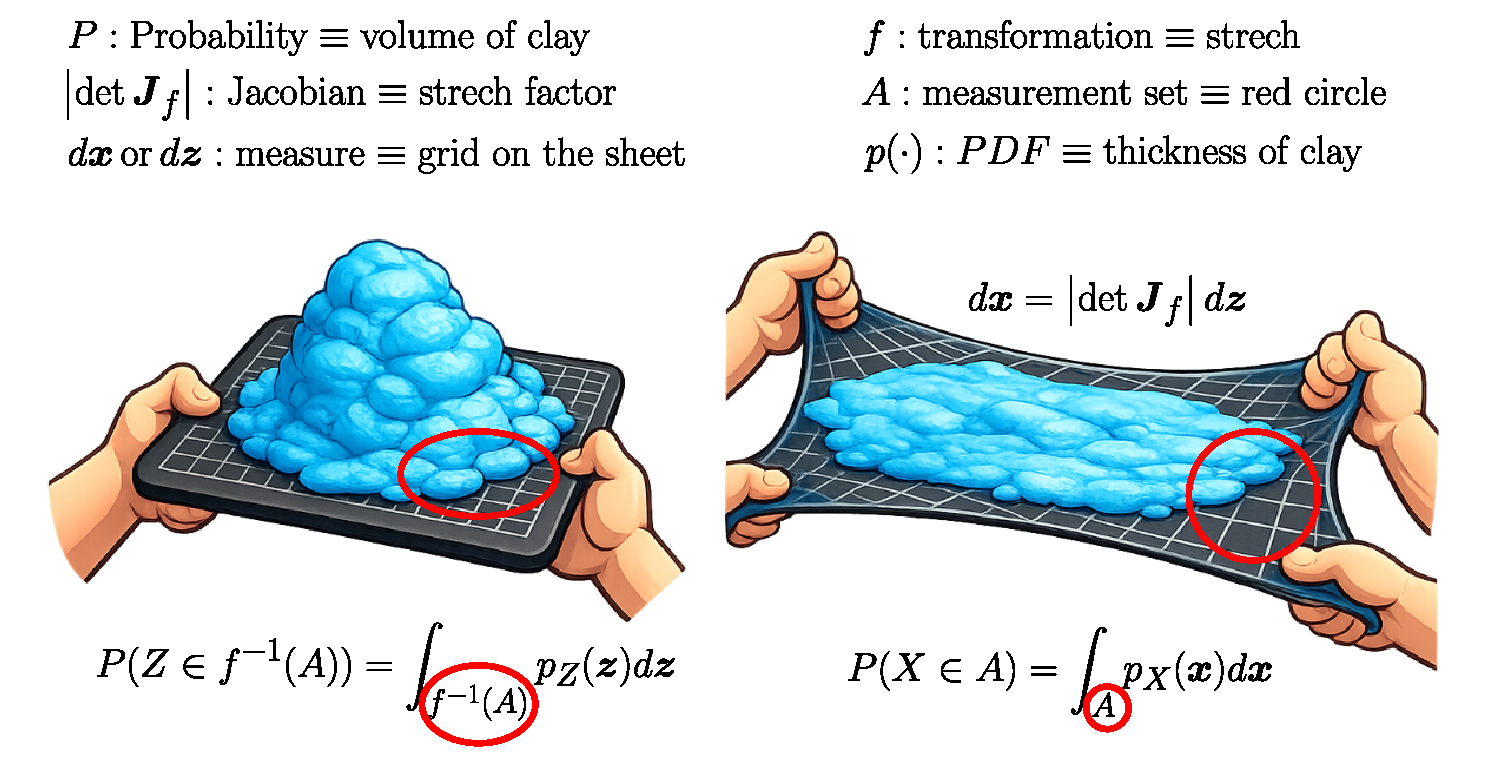
\includegraphics[width=0.9\textwidth]{figures/radon_nikodym.pdf}
    \caption[The Clay Volume Analogy for Change of Variables]{The Clay Volume Analogy for Change of Variables. Probability mass is represented as clay on a rubber sheet. Transforming the variable ($\boldsymbol{z}\to\boldsymbol{x}$) stretches the sheet. While the total amount of clay (probability $P$) remains constant, the local thickness (density $p(\cdot)$) decreases as the area increases.}
    \label{fig:rnd}
\end{figure}

In probability theory, the \textit{Radon–Nikodym derivative} \citep{DU04} provides a rigorous method to express how one probability measure changes with respect to another. In the context of continuous random variables, the \ac{PDF} is essentially the Radon–Nikodym derivative of the probability measure (probability mass of an event) with respect to the Lebesgue measure (standard geometric volume). This relationship generalizes the familiar link between a \ac{CDF} and a \ac{PDF}. To provide a physical intuition for this abstract concept, we introduce the "Clay Volume" Analogy illustrated in Figure~\ref{fig:rnd}. The Radon–Nikodym derivative corresponds to the local thickness of the clay at any given point.

For a random variable $\boldsymbol{x}$ and a measurement set $A$, the probability measure is defined by the integral of the density:
\begin{equation}
    P(X\in A)=\int_A p_X(\boldsymbol{x})d\boldsymbol{x}.
\end{equation}
To relate this to a transformed variable $\boldsymbol{z}$ via an invertible mapping (Equation~(\ref{eq:zfx})), we rely on the invariance of probability. An event occurs in $A$ for $\boldsymbol{x}$ if and only if it occurs in the pre-image $f^{-1}(A)$ for $\boldsymbol{z}$:
\begin{subequations}
    \begin{gather}
        P(X\in A)=P(Z\in f^{-1}(A)),\\
        \label{eq:intx}
        \int_A p_X(\boldsymbol{x})d\boldsymbol{x}=\int_{f^{-1}(A)}p_Z(\boldsymbol{z})d\boldsymbol{z}.
    \end{gather}
\end{subequations}
We apply the multivariate change of variables formula (Equation~\ref{eq:changeofvariables}) to the right-hand integral in Equation~(\ref{eq:intx}). This transforms the domain of integration from $f^{-1}(A)$ back to $A$, introducing the Jacobian determinant to account for local volume distortion:
\begin{equation}
    \label{eq:intz}
    \int_{f^{-1}(A)}p_Z(\boldsymbol{z})d\boldsymbol{z}=\int_A p_Z(f^{-1}(\boldsymbol{x}))\left|\det\boldsymbol{J}_{f^{-1}}(\boldsymbol{x})\right|d\boldsymbol{x}.
\end{equation}
Here, the Jacobian determinant of the inverse mapping $f^{-1}$ is related to the forward mapping by:
\begin{equation}
    \left|\det\boldsymbol{J}_{f^{-1}}(\boldsymbol{x})\right|=\left|\det\frac{\partial f^{-1}(\boldsymbol{x})}{\partial\boldsymbol{x}}\right|=\left|\det\frac{\partial\boldsymbol{z}}{\partial f(\boldsymbol{z})}\right|=\frac{1}{\left|\det\boldsymbol{J}_f(\boldsymbol{z})\right|}.
\end{equation}
By substituting (\ref{eq:intz}) into (\ref{eq:intx}), we obtain an equality of two integrals defined over the same domain $A$:
\begin{equation}
    \label{eq:integral_equality}
    \int_A p_X(\boldsymbol{x})d\boldsymbol{x}=\int_A p_Z(f^{-1}(\boldsymbol{x}))\left|\det\boldsymbol{J}_{f^{-1}}(\boldsymbol{x})\right|d\boldsymbol{x}.
\end{equation}
Crucially, Equation~(\ref{eq:integral_equality}) holds for any arbitrary measurable set $A$. In measure theory, if two continuous functions integrate to the same value over every possible subset of the domain, the functions themselves must be identical almost everywhere. Therefore, we can equate the integrands directly:
\begin{equation}
    \label{eq:xnfz}
    p_X(\boldsymbol{x}) = p_Z(f^{-1}(\boldsymbol{x}))\left|\det\boldsymbol{J}_{f^{-1}}(\boldsymbol{x})\right|.
\end{equation}
Substituting $\boldsymbol{x}$ and $\boldsymbol{z}$ with equations \ref{eq:xfz} and \ref{eq:zfx} respectively, it can also be formulated using the forward mapping $f$:
\begin{equation}
    \label{eq:znfx}
    p_Z(\boldsymbol{z}) = p_X(f(\boldsymbol{z}))\left|\det\boldsymbol{J}_f(\boldsymbol{z})\right|.
\end{equation}
These two equations define the \textbf{change of variables} formula applied to \acp{NF}. They are often formulated in logarithmic form:
\begin{mdframed}[nobreak=true,innertopmargin=-4pt,innerbottommargin=4pt,innerleftmargin=6pt,innerrightmargin=6pt]
    \begin{align}
        \label{eq:nfchangeofvariables}
        \log p_X(\boldsymbol{x}) &= \log p_Z(f^{-1}(\boldsymbol{x}))+\log\left|\det\boldsymbol{J}_{f^{-1}}(\boldsymbol{x})\right|,\\
        \log p_Z(\boldsymbol{z}) &= \log p_X(f(\boldsymbol{z}))+\log\left|\det\boldsymbol{J}_f(\boldsymbol{z})\right|.
    \end{align}
\end{mdframed}

The derivation of the probability density in Equation~(\ref{eq:znfx}) relies fundamentally on the Change of Variables theorem. Consequently, for a Normalizing Flow to be both mathematically valid and computationally tractable, the transformation $f$ cannot be arbitrary; it must satisfy three strict structural constraints:
\begin{enumerate}
    \item \textbf{Invertibility (Bijectivity):} 
    The mapping $f: Z \to X$ must be bijective. This ensures that the inverse $f^{-1}$ exists and is unique, allowing distinct data points $\boldsymbol{x}$ to be uniquely mapped to latent representations $\boldsymbol{z}$ (inference) and vice versa (sampling).
    \item \textbf{Differentiability:} 
    The function $f$ and its inverse must be differentiable. This is a prerequisite for the existence of the Jacobian matrix $\boldsymbol{J}_f$. In differential geometry, a map satisfying conditions (1) and (2) is termed a \textit{diffeomorphism}.
    \item \textbf{Computational Efficiency of the Jacobian:} 
    While the first two properties ensure mathematical validity, this third property ensures practical feasibility. Training an \ac{NF} involves maximizing the log-likelihood, which requires calculating the log-determinant of the Jacobian, $\log |\det \boldsymbol{J}_f(\boldsymbol{z})|$. 
    For an arbitrary high-dimensional function with a dimension $D$, this calculation scales with $\mathcal{O}(D^3)$. To make training efficient, Normalizing Flows are explicitly designed such that this term can be computed in linear time, $\mathcal{O}(D)$, often by restricting the Jacobian to be triangular or diagonal.
\end{enumerate}
Beyond the structural constraints of individual mappings, a powerful feature of \acp{NF} is composability \citep{papamakarios2021nf}. Given a series of transformations $f_{L}\circ\cdots\circ f_{1}$, the following equations hold:
\begin{subequations}
    \begin{gather}
        % Composition
        \boldsymbol{x} = f_L(f_{L-1}(\cdots f_{1}(\boldsymbol{z})\cdots)), \\
        % Inversion
        \label{eq:inverse_composition}
        f^{-1} = (f_L \circ \cdots \circ f_1)^{-1} = f_1^{-1} \circ \cdots \circ f_L^{-1}, \\
        % Jacobian Chain Rule
        \label{eq:jacobian_chain_rule}
        \boldsymbol{J}_{f}(\boldsymbol{z}) = \boldsymbol{J}_{f_L}(\boldsymbol{z}_{L-1}) \cdot \boldsymbol{J}_{f_{L-1}}(\boldsymbol{z}_{L-2}) \cdots \boldsymbol{J}_{f_1}(\boldsymbol{z}_0).
    \end{gather}
\end{subequations}
Equation~(\ref{eq:jacobian_chain_rule}) applies the multivariate \textbf{chain rule}. A crucial consequence for training is that the log-determinant of the Jacobian decomposes into a sum of terms:
\begin{equation}
    \log \left| \det \boldsymbol{J}_f(\boldsymbol{z}) \right| = \sum_{k=1}^{L} \log \left| \det \boldsymbol{J}_{f_k}(\boldsymbol{z}_{k-1}) \right|.
\end{equation}
This allows the total change in density to be computed by simply summing the log-determinants of each layer, enabling the construction of deep, expressive flows while maintaining linear computational complexity.

\subsubsection{Using Normalizing Flows for Modeling and Inference}
Invertibility also provides an easy way to fit \ac{NF} models by minimizing the divergence between the true data distribution and the estimated one. For a \ac{NF} with parameters $\boldsymbol{\varphi}$, the KL-divergence is given by:
\begin{equation}
    D_{\text{KL}}(p_X(\boldsymbol{x}) || p_{\boldsymbol{\varphi}}(\boldsymbol{x})) = 
    \mathbb{E}_{\boldsymbol{x} \sim p_X}[\log p_X(\boldsymbol{x})] - \mathbb{E}_{\boldsymbol{x} \sim p_X}[\log p_{\boldsymbol{\varphi}}(\boldsymbol{x})].
\end{equation}
In this objective function, the first term (the entropy of the data) depends only on the true distribution and is constant with respect to $\boldsymbol{\varphi}$. Consequently, minimizing the KL divergence is equivalent to maximizing the second term, which corresponds to the expected log-likelihood. Given a dataset $\mathcal{D} = \{\boldsymbol{x}^{(m)}\}_{m=1}^M$ drawn from $p_X(\boldsymbol{x})$, we can approximate this expectation using the sample mean (Monte Carlo simulation):
\begin{equation}
    \mathbb{E}_{\boldsymbol{x} \sim p_X}[\log p_{\boldsymbol{\varphi}}(\boldsymbol{x})] \approx \frac{1}{M}\sum_{m=1}^{M}\log p_{\boldsymbol{\varphi}}(\boldsymbol{x}^{(m)}).
\end{equation}

This confirms that minimizing the KL divergence is equivalent to \ac{MLE}. By substituting the change of variables formula (Equation~(\ref{eq:xnfz})) into the log-likelihood, we obtain the final loss function to be minimized:

\begin{align}
\label{eq:kl_nf}
\mathcal{L}(\boldsymbol{\varphi}) &= - \frac{1}{M}\sum_{m=1}^{M} \left[ \log p_{Z}(f_{\boldsymbol{\varphi}}^{-1}(\boldsymbol{x}^{(m)})) + \log \left| \det \boldsymbol{J}_{f_{\boldsymbol{\varphi}}^{-1}}(\boldsymbol{x}^{(m)}) \right| \right], \nonumber\\
&= \frac{1}{M}\sum_{m=1}^{M} \left[ \underbrace{\frac{1}{2}\left\|f_{\boldsymbol{\varphi}}^{-1}(\boldsymbol{x}^{(m)})\right\|^2_2}_{\text{inference}} \underbrace{- \log \left| \det \boldsymbol{J}_{f_{\boldsymbol{\varphi}}^{-1}}(\boldsymbol{x}^{(m)}) \right|}_{\text{preparation for generation}} \right], \quad \text{when } p_Z(\boldsymbol{z})=\mathcal{N}(\boldsymbol{0},\boldsymbol{I}).
\end{align}
The parameters $\boldsymbol{\varphi}$ are then optimized using stochastic gradient-based methods.

The loss function of \acp{NF} suggests that during training, the learned latent representation is compared with the true latent distribution, while the Jacobian determinant term ensures that this comparison is transformed back to the data space. Recalling the \ac{VAE}, the first term can be seen as inference, while the second term can be implicitly regarded as "preparation for generation". After the \ac{NF} model is trained, new data can be generated by sampling the latent variables and transforming them via the forward mapping. It is important to emphasize that \acp{NF} are conventionally trained in one direction at a time. Simultaneously bidirectional training would necessitate computing gradients through the composition of a function and its inverse, leading to problematic gradient flows of the form $\partial \mathcal{L}/\partial \boldsymbol{\varphi}_f(\boldsymbol{\varphi{f^{-1}}})$, which creates numerical instabilities and computational inefficiencies.

\subsubsection{Conditional Normalizing Flows}
\label{sec:condnf}
The ability to estimate complex densities is desirable in Bayesian inference of the posterior distribution of variables given observations $p(\boldsymbol{x}|\boldsymbol{y})$. Similar to \ac{VAE}, amortized Bayesian inference \citep{radev2021diss} is applied in \ac{NF} to achieve a general posterior estimation across all data points. Obtaining the posterior distribution is represented by a conditional density transformation via a \ac{CNF}. The change of variables for a \ac{CNF} extends the standard one (\ref{eq:xnfz}) by the condition $\boldsymbol{y}$:
\begin{equation}
    p_{X|Y}(\boldsymbol{x}|\boldsymbol{y}) = p_{Z|Y}(f^{-1}(\boldsymbol{x},\boldsymbol{y})|\boldsymbol{y})\left|\det\frac{\partial f^{-1}(\boldsymbol{x},\boldsymbol{y})}{\partial\boldsymbol{x}}\right|,
\end{equation}
where the mapping $f:Z\rightarrow X\times Y$ is bijective between $X$ and $Z$, and $\boldsymbol{z}=f^{-1}(\boldsymbol{x},\boldsymbol{y})$.

Designing such a \ac{CNF} requires addressing two key considerations in advance: (1) how to manage the conditioned latent variables, and (2) how to incorporate conditions into the flow architecture while preserving invertibility. \citeauthor{winkler2023cnf} \citeyearpar{winkler2023cnf} proposed to build the conditional prior $p_{Z|Y}(\boldsymbol{z}|\boldsymbol{y})$ as a diagonal Gaussian:
\begin{equation}
    p_{Z|Y}(\boldsymbol{z}|\boldsymbol{y}) = \mathcal{N}({\boldsymbol{z}|\mu(\boldsymbol{y}), \text{diag}[\sigma^2(\boldsymbol{y})]}).
\end{equation}
For simpler conditioning scenarios, incorporating the conditional prior could accelerate the transformation by leveraging information from the conditions. For complex conditions, summarizing the conditions through mean and variance may result in information loss, thereby degrading posterior estimation quality. This limitation likely explains why most existing work on \acp{CNF} adopts a standard Gaussian as the latent base distribution, bypassing the need for an explicitly conditioned prior and relying instead on the normalizing flows to capture conditional information.

In terms of architectures of \acp{CNF}, a direct adaptation based on the \ac{INN} is the \ac{cINN} \citep{ardizzone2019cinn}. It takes the condition as an augmented input to the neural networks. In cases of higher-dimensional conditions, such as images, \citeauthor{govinda2021cinn} \citeyearpar{govinda2021cinn} apply a staged \ac{cINN} coupled with a staged condition network, wherein the conditions are progressively processed, and each intermediate representation is fed into its corresponding \ac{cINN} block.

In scenarios involving complexly structured conditions and low-dimensional target variables, for example, parameter identification from observed time series signals, BayesFlow \citep{radev2020bayesflow} offers a general framework by extracting informative representations through a summary network and incorporating them, alongside the inputs as augmented inputs to the \ac{cINN}. This framework is particularly well-suited for parameter identification from time series observations, where the summary network is typically chosen as a time series modeling architecture, such as \ac{RNN}. The architecture is illustrated in Figure~\ref{fig:bayesflow}. Both the summary network and \ac{cINN} are optimized together by minimizing the \ac{KL}-divergence between the true posterior density and the estimated one (similar to Equation~(\ref{eq:kl_nf})):
\begin{multline}
\label{eq:kl_cnf}
D_{\text{KL}}(p_{X|Y}(\boldsymbol{x}|\boldsymbol{y})||p_{\boldsymbol{\varphi},\boldsymbol{\phi}}(\boldsymbol{x}|\boldsymbol{y}))\approx const. - \\
\frac{1}{M}\sum_{m=1}^{M}[\log p_{Z}(f_{\boldsymbol{\varphi}}^{-1}(\boldsymbol{x}^{(m)}, h_{\boldsymbol{\phi}}(\boldsymbol{x}^{(m)})))+\log\left|\det\boldsymbol{J}_{f_{\boldsymbol{\varphi}}^{-1}}(\boldsymbol{x}^{(m)},h_{\boldsymbol{\phi}}(\boldsymbol{x}^{(m)}))\right|],
\end{multline}
where $f$ is the \ac{cINN} parameterized by $\boldsymbol{\varphi}$ and $h$ is the summary network parameterized by $\boldsymbol{\phi}$.

\begin{figure}[htp!]
    \centering
    \includegraphics[width=0.85\textwidth]{figures/BayesFlow.pdf}
    \caption[BayesFlow Architecture]{ The architecture of BayesFlow. The blue arrows indicate the forward direction for training BayesFlow, while the yellow arrows indicate the reverse direction for inference. The summary network extracts informative representations from the observations, which are then fed into the \ac{cINN} alongside the target variables.}
    \label{fig:bayesflow}
\end{figure}
The joint optimization approach encourages the summary network to deliver maximally useful information to the \ac{cINN} and thus improve inference capability. In this work, we adopt the BayesFlow framework as a flexible and scalable solution for amortized Bayesian inference, adapting its summary network to accommodate diverse time series observations. This framework forms the foundation of our proposed methods for parameter identification, system dynamics modeling, and state estimation.

\subsection{Coupling Flows}\label{sec:background:coupling}
The basic idea of a coupling flow is to partition the input variables into two subsets: one subset is processed by neural networks while being passed directly to the output variables, and the other subset is combined with the processed subset through affine functions.
\begin{figure}[htp!]
    \centering
    \begin{subfigure}{0.45\textwidth}
        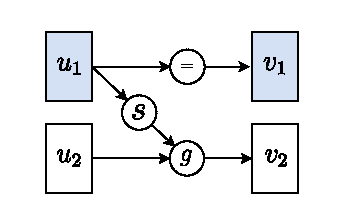
\includegraphics{figures/NICE.pdf}
        \caption[NICE Architecture]{ The architecture of a \ac{NICE} layer. $s$ is a neural network, and $g$ is an affine function.}
        \label{fig:nice}
    \end{subfigure}
    \hspace{0.02\textwidth}
    \begin{subfigure}{0.5\textwidth}
        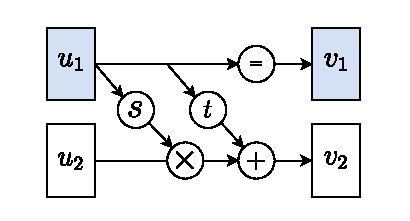
\includegraphics{figures/RealNVP.pdf}
        \caption[RealNVP Architecture]{ The architecture of a \ac{RealNVP} layer. $s$ and $t$ are neural networks. The symbol $\times$ denotes element-wise multiplication by the exponential function over the input.}
        \label{fig:realnvp}
    \end{subfigure}
    \begin{subfigure}{\textwidth}
        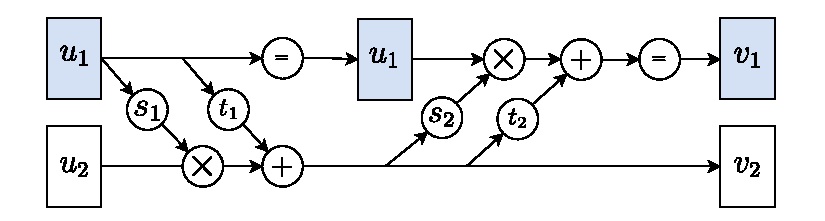
\includegraphics{figures/INN.pdf}
        \caption[INN Architecture]{ The architecture of an \ac{INN} layer. $s_1$, $s_2$, $t_1$, and $t_2$ are neural networks. The symbol $\times$ denotes element-wise multiplication by the exponential function over the input.}
        \label{fig:inn}
    \end{subfigure}
    \caption[Coupling Flow Architecture]{ The architectures of coupling flows. The input of the layer is $\boldsymbol{u}$ and the output is $\boldsymbol{v}$.}
    \label{fig:coupling}
\end{figure}

The first proposed coupling flow was \ac{NICE} \citep{dinh2015nice}. The input variables $\boldsymbol{u}$ are split into two parts $[\boldsymbol{u}_1, \boldsymbol{u}_2]$, and the corresponding output variables are $\boldsymbol{v} = [\boldsymbol{v}_1, \boldsymbol{v}_2]$. The architecture in the forward direction is formulated by the following functions:
\begin{equation}
    \boldsymbol{v}_1 = \boldsymbol{u}_1, \quad \boldsymbol{v}_2 = g(\boldsymbol{u}_2;s(\boldsymbol{u}_1)),
\end{equation}
where $s$ is a neural network and $g$ is an affine function $g(a;b)=a+b$ or $a\odot b$ (element-wise multiplication). The forward architecture is illustrated in Figure~\ref{fig:nice}.
Then, the inverse functions are easily calculated:
\begin{equation}
    \boldsymbol{u}_1 = \boldsymbol{v}_1,\quad \boldsymbol{u}_2 = g^{-1}(\boldsymbol{v}_2;s(\boldsymbol{u}_1)).
\end{equation}
From the above functions, the Jacobian matrix is:
\begin{equation}\label{eq:background:nice}
\frac {\partial \boldsymbol{v}}{\partial \boldsymbol{u}}=\begin{bmatrix}
\partial \boldsymbol{v}_1/\partial \boldsymbol{u}_1 & \partial \boldsymbol{v}_1/\partial \boldsymbol{u}_2 \\
\partial \boldsymbol{v}_2/\partial \boldsymbol{u}_1 & \partial \boldsymbol{v}_2/\partial \boldsymbol{u}_2\\
\end{bmatrix}=\begin{bmatrix}
\boldsymbol{I} & \boldsymbol{0} \\
\partial \boldsymbol{v}_2/\partial \boldsymbol{u}_1 & \partial g(\boldsymbol{u}_2;s(\boldsymbol{u}_1))/\partial \boldsymbol{u}_2\\
\end{bmatrix}
\end{equation}
Because of the triangular matrix, the determinant is $ \partial g(\boldsymbol{u}_2;s(\boldsymbol{u}_1))/\partial \boldsymbol{u}_2$.
By composing multiple coupling layers, we can construct increasingly complex hierarchical transformations. Since each coupling layer preserves a subset of its input unchanged, it is essential to alternate the roles of the partitioned subsets across successive layers. This ensures that all input dimensions are eventually processed. Analyzing the Jacobian reveals that a minimum of three coupling layers is required for full inter-dimensional interaction. In practice, we typically employ four layers to achieve sufficient expressiveness.

An improved architecture is \ac{RealNVP}, where one part of the variables is processed by two neural networks. The forward transformation is:
\begin{equation}
    \boldsymbol{v}_1 = \boldsymbol{u}_1, \quad \boldsymbol{v}_2 = \boldsymbol{u}_2\odot\exp(s(\boldsymbol{u}_1))+t(\boldsymbol{u}_1).
\end{equation}
The inverse transformation is:
\begin{equation}
    \boldsymbol{u}_1 = \boldsymbol{v}_1, \quad \boldsymbol{u}_2 = (\boldsymbol{v}_2-t(\boldsymbol{u}_1))\odot\exp(-s(\boldsymbol{u}_1)).
\end{equation}
The Jacobian determinant $\det|\partial\boldsymbol{v}/\boldsymbol{u}|$ is then $\exp(\Sigma_i s(\boldsymbol{u}_{1,i}))$.
The architecture is shown in Figure~\ref{fig:realnvp}. To interact all variables in one block, \ac{INN} \citep{ardizzone2019inn} extends \ac{RealNVP} by another coupling block of the same form, as shown in Figure~\ref{fig:inn}. 

A further enhancement of \ac{RealNVP} is Glow \citep{kingma2018glow}, which inserts an invertible normalization layer and an invertible permutation layer before affine transformation. \ac{HINT} \citep{kruse2021hint} partitions the inputs of coupling blocks recursively to construct a dense, triangular Jacobian. Another method to increase interaction among variables is \ac{MAF} \citep{papamakarios2018maf}, which can be considered as a generalized \ac{RealNVP} that leverages autoregressive transformations between variables. Apart from affine coupling, \ac{NSF} \citep{durkan2019neuralsplineflows} applies monotonic rational-quadratic spline functions, enabling more expressive and smooth transformations, but at the cost of higher complexity. 

\subsection{Residual Flows}\label{sec:resflow}
Such flows build stepwise invertible transformations between distributions, enabling tractable Jacobian calculation and density estimation. A notable drawback lies in the strict architectural constraint on coupling blocks. To relax this limitation, residual flows \citep{behrmann2019ires, chen2020resflow} introduce invertible mapping through specified residual blocks. A residual block \citep{he2015residual} takes the form $f(x)=x+F(x)$, where $F$ is a neural network. When $F$ is constrained to be Lipschitz continuous and the Lipschitz constant is smaller than 1, the function $f(x)$ is invertible. 

The definition of a Lipschitz continuous function follows the work of \citeauthor{khalil2002nonlinear} \citeyearpar{khalil2002nonlinear}.
\begin{definition}
(\textbf{Lipschitz continuous function}) A function $f:\mathbb{R}^d\rightarrow\mathbb{R}^K$, defined on some domain $dom(f)\subseteq \mathbb{R}^d$, is called $C$-Lipschitz continuous w.r.t. some $\alpha$-norm, if $\forall \boldsymbol{x}, \boldsymbol{y} \in dom(f):\left\| f(\boldsymbol{x})-f(\boldsymbol{y})\right\|_{\alpha}\leq C\left\| \boldsymbol{x}-\boldsymbol{y}\right\|_{\alpha}$. $C$ is called the Lipschitz constant of $f$ and $0<C<\inf$.
\end{definition}

\begin{lemma}\label{lem:invertibility}(\textbf{Invertibility of Residual Units}) 
    Let $f(\mathbf{x}) = \mathbf{x} + F(\mathbf{x})$. If $F$ is $C$-Lipschitz continuous with $C < 1$, then $f$ is a bijection.
\end{lemma}
\begin{proof}
    To show $f$ is invertible, we must show that for any $\mathbf{y}$, there exists a unique $\mathbf{x}$ such that $\mathbf{y} = \mathbf{x} + F(\mathbf{x})$. This can be rewritten as a fixed-point problem:
    \begin{equation}
    \mathbf{x} = \mathbf{y} - F(\mathbf{x}) = G(\mathbf{x}).
    \end{equation}
    By the definition of $G$, for any $\mathbf{x}_1, \mathbf{x}_2$:
    \begin{align}
    \left\|G(\mathbf{x}_1) - G(\mathbf{x}_2)\right\| &= \left\|(\mathbf{y} - F(\mathbf{x}_1)) - (\mathbf{y} - F(\mathbf{x}_2))\right\| \\
    &= \left\|F(\mathbf{x}_2) - F(\mathbf{x}_1)\right\| \\
    &\leq C \left\|\mathbf{x}_2 - \mathbf{x}_1\right\|.
    \end{align}
    Since $C < 1$, $G$ is a contraction mapping. According to the \textit{Banach Fixed-Point Theorem} \citep{Shukla2016}, $G$ has a unique fixed point $\mathbf{x}^*$ for every $\mathbf{y}$, implying $f$ is bijective.
\end{proof}

The residual block can be seen as an Euler discretization of an \ac{ODE} \citep{lu2020finitelayer, ruthotto2018deep, haber2017stable}, which is the foundation of continuous \acp{NF}. A simplified comparison between the residual flow, continuous flow, and flow matching is illustrated in Figure~\ref{fig:illust_flow}.

\begin{figure}[htp!]
    \centering
    \begin{subfigure}{0.32\textwidth}
        \centering
        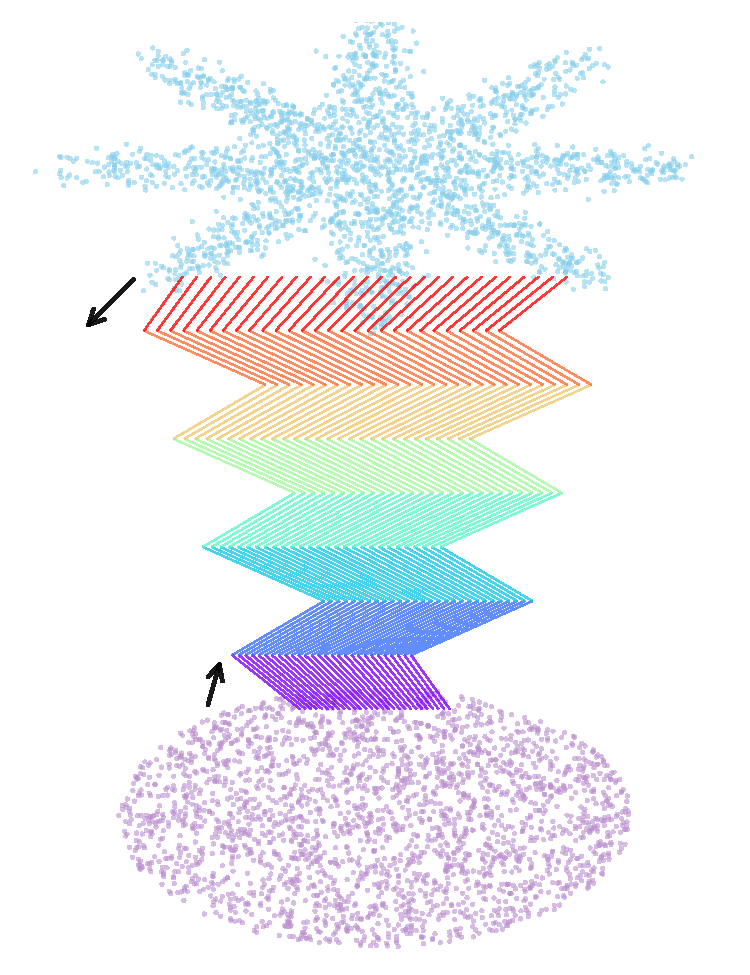
\includegraphics[width=\linewidth]{figures/residual_flow_illustration.pdf}
        \caption{Residual Flow}
        \label{fig:resflow}
    \end{subfigure}
    \hfill
    \begin{subfigure}{0.32\textwidth}
        \centering
        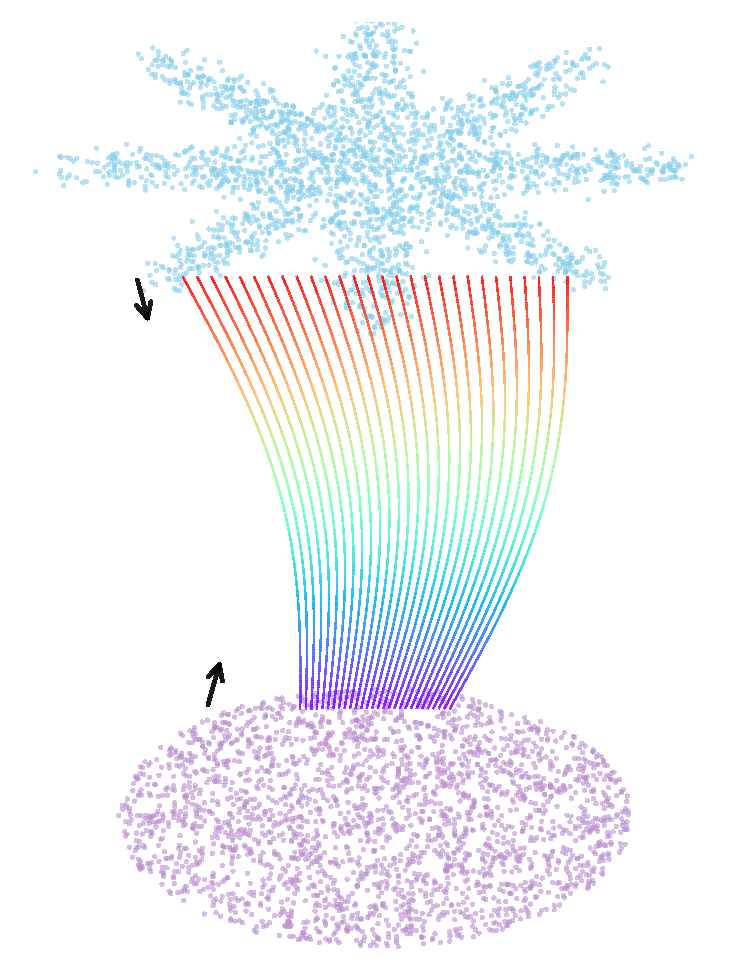
\includegraphics[width=\linewidth]{figures/continuous_flow_illustration.pdf}
        \caption{Continuous Flow}
        \label{fig:contflow}
    \end{subfigure}
    \hfill
    \begin{subfigure}{0.32\textwidth}
        \centering
        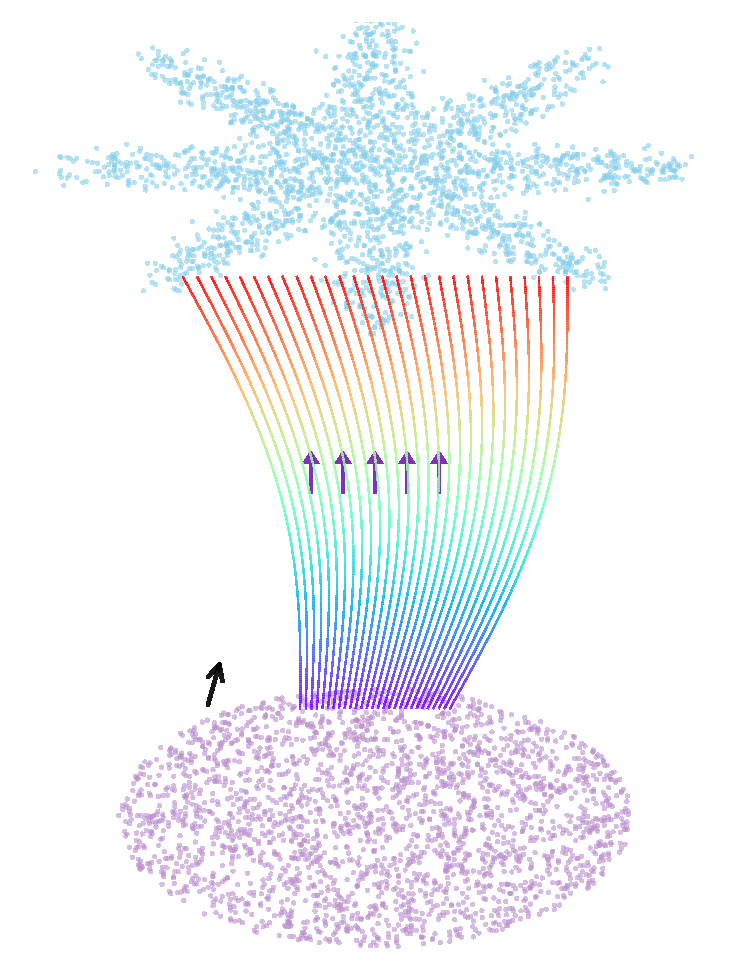
\includegraphics[width=\linewidth]{figures/flow_matching_illustration.pdf}
        \caption{Flow Matching}
        \label{fig:flowmatch}
    \end{subfigure}
    \caption[Illustration of three Flows]{Illustration of the Residual Flow, Continuous Flow, and Flow Matching. The bottom point cloud is the base distribution in the latent space, while the top one in the star shape is the target distribution in the data space. The residual flow and continuous flow are trained from the data to latent space and sampled from latent to the data space, while Flow Matching is trained by learning the vector field and sampled from the latent to the data space. The reverse direction is not used by Flow Matching.}
    \label{fig:illust_flow}
\end{figure}

\subsection{Continuous Flows}\label{sec:cnf}
When the transformation from latent space to data space is modeled by a continuous dynamical system, the \ac{NF} is called a \textit{continuous \ac{NF}}. The continuous dynamical system can be formulated by a Neural \ac{ODE}, which is introduced as follows.

\subsubsection{Neural Ordinary Differential Equations}
For a dynamical system with states $\boldsymbol{h}$, an \ac{ODE} is:
\begin{equation}
    \frac{d\boldsymbol{h}(t)}{dt} = f(\boldsymbol{h}(t), t; \boldsymbol{\varphi}),
\end{equation}
where $\boldsymbol{\varphi}$ denotes system parameters. When the \ac{ODE} is modeled by neural networks, it becomes a Neural \ac{ODE} \citep{chen2019node}. Given the initial state $\boldsymbol{h}(0)$, the final state $\boldsymbol{h}(T)$ is the solution of the initial value problem at the time step $T$ using a numerical solver. The loss function of training a Neural \ac{ODE} is:
\begin{equation}
    \mathcal{L}(\boldsymbol{h}(T))=\mathcal{L}(\int_0^Tf(\boldsymbol{h}(t), t; \boldsymbol{\varphi})dt),
\end{equation}
where $f$ is a neural network parameterized by $\boldsymbol{\varphi}$.
A straightforward application of Neural \acp{ODE} is learning continuous time-series models. Moreover, when the time step is interpreted as architectural depth, the distributional transformation in \acp{NF} can also be constructed with a Neural \ac{ODE}. The Neural \ac{ODE} replaces an infinite number of transformations by change of variables with a single neural network, which represents the derivative of transformation at each depth. This enables more efficient and expressive probabilistic modeling and inference.

Taking $\mathcal{U}_\tau$ as the state variable at flow time $\tau$, we define a continuous \ac{NF} as a Neural \ac{ODE}:
\begin{equation}
    \label{eq:cnfode}
    \frac{d\mathcal{U}_\tau}{d\tau}=f(\mathcal{U}_\tau,\tau;\boldsymbol{\varphi}),
\end{equation}
where $\mathcal{U}_\tau$ follows the density $p(\mathcal{U}_\tau)$ at an instantaneous step $\tau\in[\tau_0, \tau_1]$. The \ac{NF} $f$ is parameterized by $\boldsymbol{\varphi}$.
To apply the Neural \ac{ODE} as continuous \acp{NF}, the function $f$ should be uniformly Lipschitz continuous in the states $\mathcal{U}_\tau$ and continuous in depth $\tau$. 

The Lipschitz condition guarantees that there exists a unique solution curve for every initial condition $\mathcal{U}_0:=\boldsymbol{z}$. This is known as the Picard–Lindel\"of theorem \citep{coddington1955theory}. If the dynamics function $f$ is smooth, then it is a \textit{diffeomorphism}, which means we can recover the same $\mathcal{U}_0$ by running the \ac{ODE} backward. Recalling the residual flows, where the Lipschitz constant must be smaller than 1 (see \ref{sec:resflow}), invertibility is ensured naturally by a smooth and Lipschitz continuous \ac{ODE}. In practice, neural networks with smooth continuous activation functions satisfy this requirement.

A central technical challenge in training continuous-depth networks lies in executing reverse-mode differentiation (backpropagation) through the ODE solver. Two primary strategies exist for this task. The first is the backward auto-differentiation (\textit{discretize-then-optimize}), which differentiates directly through the operations of the numerical solver. While this method is numerically stable and standard for stiff differential equations, it typically incurs a high memory cost as it requires storing intermediate states of the solver operations.

To mitigate this memory bottleneck, the continuous adjoint method \citep{Bittner1963, adjoint1963, chen2019node} is often employed (\textit{optimize-then-discretize}). This method computes gradients by solving an augmented ODE backward in time. Specifically, instead of storing intermediate states, the solver reconstructs the state trajectory backward from the final time point, effectively re-solving the dynamics in reverse alongside the adjoint state. This approach reduces memory cost to $\mathcal{O}(1)$ with respect to integration time. However, because the system dynamics must be evaluated a second time during this reconstruction, it results in increased computational runtime. This trade-off makes the adjoint method ideal for high-dimensional variables and long sequences, but computationally slower for models with expensive architecture dynamics.

\subsubsection{Continuous Normalizing Flows}
In addition to the ODE \ref{eq:cnfode}, the log-density of states changes according to another \ac{ODE}, the \textbf{instantaneous change-of-variables formula} \citep{chen2019node}:
\begin{equation}
    \label{eq:instchangeofvar}
    \frac{\partial\log p(\mathcal{U}_\tau)}{\partial \tau}=-\text{Tr}(\frac{\partial f(\mathcal{U}_\tau,\tau;\boldsymbol{\varphi})}{\partial\mathcal{U}_\tau}).
\end{equation}
Directly calculating the trace is computationally expensive. For $B$ backward passes to get the diagonal, $\mathcal{O}(B)$ computational cost and $\mathcal{O}(B^2)$ memory cost are required. Alternatively, the trace can be approximated through Skilling-Hutchinson trace estimator \citep{Skilling1989,Hutchinson01011990,adams2018adams}:
\begin{equation}
    \text{Tr}(\frac{\partial f}{\partial \mathcal{U}_\tau})=\mathbb{E}_{p(\boldsymbol{\epsilon})}[\boldsymbol{\epsilon}^T\frac{\partial f}{\partial \mathcal{U}_\tau}\boldsymbol{\epsilon}],
\end{equation}
where $\boldsymbol{\epsilon}$ is a noise vector sampled from a standard normal distribution and kept unchanged to maintain determinism of the \ac{ODE}. The part of vector-Jacobian product $\boldsymbol{\epsilon}^T\partial f/\partial \mathcal{U}_\tau$ is computed with automatic differentiation. In this way, the computational cost is reduced to $\mathcal{O}(1)$ with respect to the number of backward passes (one backward pass for each trace approximation). There is no need to store the full Jacobian matrix. The trade-off is that the estimator introduces variance, as it yields a stochastic approximation of the trace rather than the exact value; in practice, one or a few samples per step are typically sufficient to keep training stable.

For a continuous \ac{NF} between the data distribution $p(\mathcal{U}_{1})=p_X(\boldsymbol{x})$ and the latent distribution $p(\mathcal{U}_0)=\mathcal{N}(\boldsymbol{0}, \boldsymbol{I})$, we define the augmented states as $[\mathcal{U}_\tau, \log p_X(\boldsymbol{x})-\log p(\mathcal{U}_\tau)]$. In the original formulation \citep{grathwohl2018ffjord}, the second term is $\log p(\mathcal{U}_\tau)$ itself; in that case, one must still calculate $\log p_X(\boldsymbol{x})-\log p(\mathcal{U}_\tau)$. The difference-based formulation used here yields a consistent form for both initial values and solutions. The total dynamics becomes:
\begin{equation}
    \frac{d}{d\tau}\begin{bmatrix}
        \mathcal{U}_\tau \\
        \log p_X(\boldsymbol{x}) - \log p(\mathcal{U}_\tau)
        \end{bmatrix}
        =
        \begin{bmatrix}
        f(\mathcal{U}_\tau, \tau; \boldsymbol{\varphi}) \\
        \text{Tr}\left(\frac{\partial f}{\partial \mathcal{U}_\tau}\right)
        \end{bmatrix}
\end{equation}
Then, building the continuous \ac{NF} is equivalent to solving the initial value problem \citep{grathwohl2018ffjord}:
\begin{equation}
\underbrace{\begin{bmatrix}
\mathcal{U}_0 \\
\log p_X(\boldsymbol{x}) - \log p(\mathcal{U}_0)
\end{bmatrix}}_{\text{solutions}}
=
\underbrace{\begin{bmatrix}
    \mathcal{U}_1=\boldsymbol{x} \\
\log p_X(\boldsymbol{x}) - \log p(\mathcal{U}_1)=0
\end{bmatrix}}_{\text{initial values}}
+\int_{1}^{0}\underbrace{\begin{bmatrix}
f(\mathcal{U}_\tau, \tau; \boldsymbol{\varphi}) \\
\text{Tr}\left(\frac{\partial f}{\partial \mathcal{U}_\tau}\right)
\end{bmatrix}}_{\text{dynamics}}d\tau.
\end{equation}
It is worth noting that the dynamics are integrated backward from $\tau=1$ to $\tau=0$, meaning from the data side to the latent side. The flow time span can also be optimized to further improve the computational efficiency \citep{du2022toflow}.

Continuous \acp{NF} release the architectural constraints of discrete flows, allowing more flexible and expressive density estimation through the integration of Neural \acp{ODE}. This improved expressiveness, however, comes at a cost: computing the Jacobian trace and the associated ODE integrals is significantly more expensive than in stacked coupling flows.

\subsection{Flow Matching}
\label{sec:flowmatching}
\ac{FM} \citep{lipman2023flowmatching} is a recent approach for training continuous \acp{NF}. The key idea is to learn a vector field that directly matches the stepwise transport (infinitesimal transport) between the data distribution and the latent distribution. This is achieved by minimizing the expected squared error between the learned vector field and the true velocity field defined by the optimal transport plan. The optimal transport plan is typically a linear interpolation between the latent samples $\mathcal{U}_0$ and the data samples $\boldsymbol{x}=\mathcal{U}_1$:
\begin{equation}
    \boldsymbol{v}^{OT}(\mathcal{U}_\tau, \tau) = \frac{\mathcal{U}_1-\mathcal{U}_0}{1 - 0}.
\end{equation}
Along this path, the marginal distribution at flow time $\tau$ is denoted $p_t(\mathcal{U}_\tau)$. For the linear interpolation with $\mathcal{U}_\tau = (1-\tau)\,\mathcal{U}_0 + \tau\,\boldsymbol{x}$, where $\mathcal{U}_0 \sim \mathcal{N}(\boldsymbol{0}, \boldsymbol{I})$ (latent distribution) and $\boldsymbol{x} \sim p_X(\boldsymbol{x})$ (data distribution), $p_t(\mathcal{U}_\tau)$ is the joint distribution through the interpolation:
\begin{equation}
    p_t(\mathcal{U}_\tau) = (1-\tau)\,p(\mathcal{U}_0) + \tau\,p_X(\boldsymbol{x}).
\end{equation}
Thus, sampling $\mathcal{U}_\tau \sim p_t(\mathcal{U}_\tau)$ amounts to drawing a random point on the transport path at flow time $\tau$.  The training objective is formulated as:
\begin{equation}
    \mathcal{L}(\boldsymbol{\varphi}) = \mathbb{E}_{\tau\sim\mathbb{U}(0,1),\;\mathcal{U}_\tau\sim p_t(\mathcal{U}_\tau)}\left[\left\|v_{\boldsymbol{\varphi}}(\mathcal{U}_\tau, \tau) - \boldsymbol{v}^{OT}(\mathcal{U}_\tau, \tau)\right\|^2\right],
\end{equation}
where $v_{\boldsymbol{\varphi}}(\mathcal{U}_\tau, \tau)$ is the learned vector field parameterized by $\boldsymbol{\varphi}$, and $\boldsymbol{v}^{OT}(\mathcal{U}_\tau, \tau)$ is the true velocity field derived from the optimal transport plan. Simply put, the \ac{FM} loss regresses the vector field $\boldsymbol{v}^{OT}$ with a neural network $v_{\boldsymbol{\varphi}}$. Upon reaching zero loss, the learned continuous \ac{NF} model will generate data samples by integrating the learned vector field from $\tau=0$ to $\tau=1$. 

The main difference from other \acp{NF} is that \ac{FM} is not trained by maximizing likelihood via change of variables between distributions. Instead, it focuses on learning the vector field that defines the continuous transformation between distributions. This approach avoids the computational overhead of solving \acp{ODE} during training, making it more efficient and scalable to high-dimensional data. However, \ac{FM} cannot be directly applied to exact density estimation because it does not transform the data distribution into a known latent distribution. The sample density it generates is only an approximation of the data density. For exact estimation, \ac{FM} must invert the generative process via a backward \ac{ODE}, which makes it computationally heavier than the single-pass inference of other \acp{NF}.

\subsection{Diffusion Models}
\label{sec:diffusionmodels}
Diffusion models are another major family of \acp{DGM} and have gained increasing attention because of their extraordinary expressive power \citep{sohl2015deep,ho2020ddpm,song2021scorebased}. They are closely related to \ac{FM}: both define an artificial flow time along the transformation from a latent noise distribution to the data distribution, and both learn a neural field that drives samples from the source side to the data side. The main difference is that \ac{FM} learns a deterministic transport velocity $v_{\boldsymbol{\varphi}}(\mathcal{U}_\tau,\tau)$, whereas diffusion models usually learn the reverse of a stochastic noising process, either through a noise-prediction network or through a score field.

In most diffusion-model literature, diffusion time is written in the opposite direction from the flow-matching convention in Section~\ref{sec:flowmatching}: the forward noising process starts from data at $t=0$ and ends at noise at $t=T$, while generation runs backward. To keep the notation consistent in this work, we use a scaled flow time $\tau\in[0,1]$ with $\tau=0$ denoting noise and $\tau=1$ denoting data.

\ac{DDPM} \citep{ho2020ddpm} defines a discrete Markov chain that gradually adds Gaussian noise to data. The noise-adding process is
\begin{equation}
    q(\mathcal{U}_{\tau}|\mathcal{U}_{\tau-1}) = \mathcal{N}\left( \mathcal{U}_{\tau}; \sqrt{1-\beta_\tau} \mathcal{U}_{\tau-1}, \beta_\tau\boldsymbol{I} \right),
\end{equation}
where $\beta_\tau$ is a prescribed noise schedule. After many steps, the distribution approaches a standard Gaussian. The generative model $\epsilon_{\boldsymbol{\varphi}}$ learns the reverse transition $p_{\boldsymbol{\varphi}}(\mathcal{U}_{\tau-1}|\mathcal{U}_{\tau})$ by predicting the added noise. The loss function is simply the mean-squared error between the predicted noise and the true noise:
\begin{equation}
    \mathcal{L}(\boldsymbol{\varphi}) = \mathbb{E}_{\tau\sim\mathbb{U}(0,1),\;\mathcal{U}_\tau\sim p_\tau(\mathcal{U}_\tau)}\left[\left\|\epsilon_{\boldsymbol{\varphi}}(\mathcal{U}_{\tau},\tau)-\epsilon\right\|^2\right].
\end{equation}
After training, the generative process is performed by sampling from the learned reverse transition $p_{\boldsymbol{\varphi}}(\mathcal{U}_{\tau-1}|\mathcal{U}_{\tau})$ from the noise side to the data side, where the noise is gradually removed.

\acp{SBM} extend this idea to continuous time and describe generation through \acp{SDE} \citep{song2021scorebased}. An \ac{SDE} that perturbs data into noise is defined as
\begin{equation}
    d\mathcal{U}_\tau
    =
    f(\mathcal{U}_\tau,\tau)d\tau
    +
    g(\tau)d\mathit{W}_\tau,
    \quad
    \mathcal{U}_0\sim p_X(\boldsymbol{x}),
\end{equation}
where $\tau$ denotes diffusion time in the standard noising direction, $f(\mathcal{U}_\tau,\tau)$ is the drift term, $g(\tau)$ is the diffusion coefficient, and $\mathit{W}_\tau$ is a standard Wiener process. In the reverse-time process, the drift term of the \ac{SDE} has to be compensated by a score function $\nabla_{\mathcal{U}_\tau}\log p_\tau(\mathcal{U}_\tau)$, which is learned by a neural network $s_{\boldsymbol{\varphi}}$. The generative process is then defined by the reverse-time \ac{SDE}:
\begin{equation}
    d\mathcal{U}_\tau = \left[f(\mathcal{U}_\tau,\tau)-g(\tau)^2\nabla_{\mathcal{U}_\tau}\log p_\tau(\mathcal{U}_\tau)\right]d\tau + g(\tau)d\mathit{W}_\tau.
\end{equation}                                                                                                       

Similar to the \ac{DDPM}, the training objective is to minimize the expected squared error between the learned score function and the true score function. Once the generative model $s_{\boldsymbol{\varphi}}$ is trained, generation is performed by integrating from the noise side toward the data side. 

In contrast to \ac{FM}, diffusion models learn a stochastic generative process, which can represent more flexible intermediate distributions and often provides stronger mode coverage for complex data. However, this comes at a much higher computational cost, as both the iterative noise-removal procedure in \ac{DDPM} and the numerical \ac{SDE}-solving procedure in \acp{SBM} require many sequential function evaluations during sampling.

\subsection{Stochastic Interpolant}\label{sec:background:si}
The previously introduced \ac{FM} and diffusion models have a similar design. They both predefine a transformation from latent to data space, and then learn the transformation function. After training, new data samples are generated by integrating the learned function. This design is unified by the definition: Stochastic Interpolant \citep{albergo2025si}.

Let $\mathcal{U}_\tau$ denote a trajectory-valued random variable defined over the artificial flow time interval $\tau\in[0,1]$. This variable is distinct from the physical state process $x_t$ used in dynamical systems, where $t$ denotes system time.
\begin{definition}
Given two probability density functions $p_0, p_1:\mathbb{R}^d\rightarrow\mathbb{R}_{\geq 0}$, a stochastic interpolant between $p_0$ and $p_1$ is a stochastic process $\mathcal{U}_\tau$ of the form
\begin{equation}
    \mathcal{U}_\tau = \mathcal{I}(\tau,\mathcal{U}_0,\mathcal{U}_1) + \gamma(\tau) \epsilon,\quad \epsilon \sim \mathcal{N}(0, \boldsymbol{I}_d),\quad \tau \in [0,1].
\end{equation}
Here,
\begin{enumerate}
    \item $\mathcal{I}(\tau,\mathcal{U}_0,\mathcal{U}_1)$ is a deterministic interpolation function satisfying $\mathcal{I}(0,\mathcal{U}_0,\mathcal{U}_1)=\mathcal{U}_0$ and $\mathcal{I}(1,\mathcal{U}_0,\mathcal{U}_1)=\mathcal{U}_1$, together with smoothness and regularity conditions that yield well-defined flow dynamics;
    \item $\gamma(\tau)$ is a noise schedule satisfying $\gamma(0)=\gamma(1)=0$ and $\gamma(\tau)>0$ for $\tau\in(0,1)$, so that stochastic perturbations vanish at the endpoints and remain well behaved in the interior;
    \item $\mathcal{U}_\tau$ has marginal distribution $p_\tau$ for each $\tau$, with $p_\tau$ continuously deforming from $p_0$ to $p_1$ as $\tau$ increases from $0$ to $1$;
    \item $\mathcal{U}_0$ and $\mathcal{U}_1$ are random variables with distributions $p_0$ and $p_1$, respectively, and are independent of the noise $\epsilon$.
\end{enumerate}
\end{definition}

\begin{figure}[ht]
    \centering
    \includegraphics[width=\textwidth]{figures/Stochastic_interpolant.pdf}
    \caption[Schematic of the stochastic interpolant framework]{Schematic of the stochastic interpolant framework. The interpolation function $I$ and noise schedule $\gamma$ determine the stochastic process and its associated dynamics, thereby unifying several generative modeling frameworks.}
    \label{fig:stochastic_interpolant}
\end{figure}

This framework connects flow matching, continuous normalizing flows, diffusion models, score-based generative models, Schr\"{o}dinger bridges, and entropy-regularized optimal transport. Figure~\ref{fig:stochastic_interpolant} provides a schematic overview. Its flexibility makes it possible to design stochastic processes tailored to a specific application or data distribution.

\section{From Bayesian Inference to Control}
This section bridges the Bayesian inference methodologies discussed above to their practical applications in control engineering. We first review how Bayesian approaches are employed for system identification and state estimation. Next, we introduce \acf{MPC}, which is a widely used model-based control method for optimal decision-making based on the system identification results. Finally, we discuss \acf{RL} as a data-driven control paradigm, highlighting its ability to learn control policies directly from interactions with the environment without requiring explicit system models. Together, these approaches illustrate the synergy between Bayesian inference and modern control strategies, enabling robust and adaptive solutions for complex dynamical systems.

\subsection{Bayesian System Identification}
An essential goal of system modeling and identification is to provide a rigorous framework for predicting and controlling the future evolution of system outputs. For any control strategy, the decision-maker needs to predict how the system will behave under any possible control input. Consider a discrete-time dynamical system with inputs $\boldsymbol{u}_{n}$ and outputs $\boldsymbol{y}_{n}$ at time $t_n$. The system evolution is governed by a (possibly stochastic) transition function:
\begin{equation}
    \boldsymbol{y}_{n} = g(\boldsymbol{u}_{n}, \mathcal{D}_{0:(n-1)}; \boldsymbol{\theta}) + \boldsymbol{\epsilon}_n,
\end{equation}
where $g$ is the system function, $\boldsymbol{\theta}$ are unknown parameters, $\mathcal{D}_{0:(n-1)}$ denotes the history of input-output pairs up to time $t_{n-1}$, and $\boldsymbol{\epsilon}_n$ is process or measurement noise. Here, we apply the same-time convention ($\boldsymbol{u}_{n}\rightarrow \boldsymbol{y}_{n}$) instead of the one-step-delaying convention ($\boldsymbol{u}_{n}\rightarrow \boldsymbol{y}_{n+1}$). Given this setup, the joint probability distribution of the future input-output sequence from $t_1$ to $t_N$, conditioned on the initial data $\mathcal{D}_{0}$, can be factorized using the chain rule of probability \citep{BayesSysId1981}:
\begin{equation}
    p(\mathcal{D}_{1:N}|\mathcal{D}_{0})=\prod _{n=1}^{N}p(\boldsymbol{y}_{n}|\boldsymbol{u}_{n}, \mathcal{D}_{0:(n-1)})p(\boldsymbol{u}_{n}|\mathcal{D}_{0:(n-1)}),
\end{equation}
where $\mathcal{D}_{n}=\{\boldsymbol{u}_{n}, \boldsymbol{y}_{n}\}$ denotes the input-output pair at time step $t_n$.
The conditional probability density $p(\boldsymbol{u}_{n}|\mathcal{D}_{0:(n-1)})$ describes the process of determining the input $\boldsymbol{u}_{n}$ on the basis of the known past history. The left-hand term $p(\boldsymbol{y}_{n}|\boldsymbol{u}_{n}, \mathcal{D}_{0:(n-1)})$ represents the dependence of the output on the corresponding input and the known past history, which can be interpreted as the system function $g$. Identifying this system consists of two steps: model selection and parameter identification. The process of finding the most plausible model from a group of candidates is model selection. System identification then focuses on inferring the parameters of the chosen system model.
\subsubsection{Bayesian Model Selection}
Among different model structures $\{\mathcal{M}_i\}$, $i=1,\ldots,|\mathcal{M}|$, the probability density of the model $\mathcal{M}_i$ given the data $\mathcal{D}$ measures whether the model is suitable for the dataset, which can also be written using Bayes’ theorem:
\begin{equation}
    p(\mathcal{M}_i|\mathcal{D})=\frac{p(\mathcal{D}|\mathcal{M}_i)p(\mathcal{M}_i)}{p(\mathcal{D})}.
\end{equation}
Model selection is also known as model comparison. The relative probability density of two different models given the same data $\mathcal{D}$ is:
\begin{equation}
    \frac{p(\mathcal{M}_i|\mathcal{D})}{p(\mathcal{M}_j|\mathcal{D})} = \frac{p(\mathcal{D}|\mathcal{M}_i)p(\mathcal{M}_i)}{p(\mathcal{D}|\mathcal{M}_j)p(\mathcal{M}_j)}.
\end{equation}
Since a model has multiple undetermined parameters, the distribution $p(\mathcal{D}|\mathcal{M})$ is obtained by integrating over all parameter variants. This integral is usually intractable. Instead, \ac{DIC} \citep{Spiegelhalter2002,Spiegelhalter2014, li2025DIC} is applied as the model selection criterion. A deviance is defined as follows:
\begin{equation}
    \text{dev}(\boldsymbol{\theta}) = -2\log p(\mathcal{D}|\boldsymbol{\theta}, \mathcal{M}),
\end{equation}
where $\boldsymbol{\theta}$ denotes the parameters of the model $\mathcal{M}$. Then, the \ac{DIC} is defined as:
\begin{equation}
    \text{DIC}(\mathcal{M}) = \mathbb{E}_{\mathcal{M}}[\text{dev}(\boldsymbol{\theta})] + P_D(\mathcal{M}),
\end{equation}
where the first term is interpreted as a Bayesian measure of model fit:
    \begin{equation}
        \mathbb{E}_{\mathcal{M}}[\text{dev}(\boldsymbol{\theta})] = \int p(\boldsymbol{\theta}|\mathcal{D}, \mathcal{M})\text{dev}(\boldsymbol{\theta})d\boldsymbol{\theta},
    \end{equation}
and the second term is used to measure the model complexity:
    \begin{equation}
        P_D(\mathcal{M}) = \mathbb{E}_{\mathcal{M}}[\text{dev}(\boldsymbol{\theta})] - \text{dev}(\overline{\boldsymbol{\theta}}),\quad \overline{\boldsymbol{\theta}}=\int p(\boldsymbol{\theta}|\mathcal{D},\mathcal{M})\boldsymbol{\theta}d\boldsymbol{\theta}.
    \end{equation}
The posterior $p(\boldsymbol{\theta}|\mathcal{D},\mathcal{M})$ is obtained by \ac{MCMC}.
\ac{DIC} balances the goodness of fit (how well the model explains the data) and the model complexity (the number of parameters in the model). A lower \ac{DIC} value indicates better model fit for the given dataset. 

\subsubsection{Bayesian Parameter Identification}
For parameter identification, we restrict the discussion to a simpler model class where the output depends only on the current input and parameters, without explicit history dependence (i.e., a memoryless or static mapping). We define the chosen system model with unknown parameters $\boldsymbol{\theta}$:
\begin{equation}
    \boldsymbol{y}_n=f(\boldsymbol{u}_n, \boldsymbol{\theta})+\boldsymbol{\epsilon}_n.
\end{equation}
The optimal parameters are selected by \ac{MAP} estimation:
\begin{equation}
    \boldsymbol{\theta}^*_{MAP}=\arg \max_{\boldsymbol{\theta}}p(\boldsymbol{\theta}|\mathcal{D}).
\end{equation}
Applying Bayes' rule (\ref{eq:bayes}), it becomes:
\begin{equation}
    \boldsymbol{\theta}^*_{MAP}=\arg \max_{\boldsymbol{\theta}}\left[\prod_{n=1}^{N} p(\boldsymbol{y}_n|\boldsymbol{u}_n,\boldsymbol{\theta})\right]p(\boldsymbol{\theta}),
\end{equation}
where $\mathcal{D}=\{(\boldsymbol{u}_n,\boldsymbol{y}_n)\}_{n=1}^{N}$ and $p(\mathcal{D})$ is dropped because it is constant with respect to $\boldsymbol{\theta}$. The noise $\boldsymbol{\epsilon}_n$ is commonly assumed to be Gaussian. Thus, the distribution $p(\boldsymbol{y}_n|\boldsymbol{u}_n,\boldsymbol{\theta})$ has a closed form, which makes this term equivalent to a weighted mean squared error. The prior density term $p(\boldsymbol{\theta})$ acts as $L2$ regularization.
In addition to parameter estimates, confidence intervals for the parameters can also be obtained from the posterior distribution.

\subsection{Bayesian State Estimation}
The basic idea of Bayesian state estimation is to apply the estimated posterior of system parameters as a prior and update the posterior with new data \citep{bayesestimation}. State estimation involves inference of the internal system states, which are not directly measurable. Expressed in a probabilistic framework, the goal of state estimation is to infer the posterior distribution of the states given observations $p(\boldsymbol{x}_{0:n}|\boldsymbol{y}_{1:n})$. Assuming a Markovian system, the posterior of the state chain is factorized as:
\begin{equation}
    \begin{split}
        p(\boldsymbol{x}_{0:n}|\boldsymbol{y}_{1:n})&=p(\boldsymbol{x}_{0:n}|\boldsymbol{y}_{n}, \boldsymbol{y}_{1:n-1})\\
        &=\frac{\textcolor{blue}{p(\boldsymbol{y}_n|\boldsymbol{x}_{0:n}, \boldsymbol{y}_{1:n-1})}\,p(\boldsymbol{x}_{0:n}|\boldsymbol{y}_{1:n-1})}{\textcolor{blue}{p(\boldsymbol{y}_n|\boldsymbol{y}_{1:n-1})}} \quad\text{\textcolor{blue}{[Bayes' rule]}} \\
        &=\frac{\textcolor{ForestGreen}{p(\boldsymbol{y}_n|\boldsymbol{x}_n)}\,p(\boldsymbol{x}_{0:n}|\boldsymbol{y}_{1:n-1})}{p(\boldsymbol{y}_n|\boldsymbol{y}_{1:n-1})} \quad\text{\textcolor{ForestGreen}{[Markov property]}} \\
        &=\frac{p(\boldsymbol{y}_n|\boldsymbol{x}_n)\,\textcolor{Sepia}{p(\boldsymbol{x}_{n}|\boldsymbol{x}_{n-1})}}{p(\boldsymbol{y}_n|\boldsymbol{y}_{1:n-1})}\,\textcolor{Sepia}{p(\boldsymbol{x}_{0:n-1}|\boldsymbol{y}_{1:n-1})}, \quad\text{\textcolor{Sepia}{[recursion]}}
    \end{split}
\end{equation}
where $p(\boldsymbol{x}_{n}|\boldsymbol{x}_{n-1})$ is referred to as \textit{evolution model}, or \textit{state transition model}, and $p(\boldsymbol{y}_n|\boldsymbol{x}_n)$ is called an \textit{observation model}, or \textit{measurement model}. The posterior $p(\boldsymbol{x}_{0:n-1}|\boldsymbol{y}_{1:n-1})$ is the result of the previous time step. Once the observation $\boldsymbol{y}_n$ is received, the term $p(\boldsymbol{y}_n|\boldsymbol{y}_{1:n-1})$ is a constant with respect to $\boldsymbol{x}_{0:n-1}$. Thus, it acts as a normalization factor. The equation above describes a recursive process of state estimation. States are indexed $0:n$ (including the initial $\boldsymbol{x}_0$); observations $1:n$ (no observation at step zero). The prior $p(\boldsymbol{x}_0)$ is the base case of the recursion.
\subsubsection{Bayesian Filters}
\label{sec:bayesfilter}
When only one state $\boldsymbol{x}_{n}$ is considered at a time, the problem is called marginal state estimation, or filtering. The equation becomes:
\begin{equation}
    \label{eq:bayesfilter}
    \begin{split}
        p(\boldsymbol{x}_{n}|\boldsymbol{y}_{1:n})&=\frac{\textcolor{blue}{p(\boldsymbol{y}_n|\boldsymbol{x}_n)}\,p(\boldsymbol{x}_{n}|\boldsymbol{y}_{1:n-1})}{p(\boldsymbol{y}_n|\boldsymbol{y}_{1:n-1})} \quad\text{\textcolor{blue}{[update]}}\\
        &=\frac{\textcolor{blue}{p(\boldsymbol{y}_n|\boldsymbol{x}_n)}}{p(\boldsymbol{y}_n|\boldsymbol{y}_{1:n-1})}\textcolor{ForestGreen}{\int p(\boldsymbol{x}_{n}|\boldsymbol{x}_{n-1})p(\boldsymbol{x}_{n-1}|\boldsymbol{y}_{1:n-1})d\boldsymbol{x}_{n-1}.} \quad\text{\textcolor{ForestGreen}{[prediction]}}.
    \end{split}
\end{equation}
From this equation, the terms with $\boldsymbol{y}_n$ (a new observation) are separated from the terms with $\boldsymbol{x}_{n-1}$ (the previous state). The first part is the update step, which incorporates the new observation $\boldsymbol{y}_n$ to refine the belief about the current state $\boldsymbol{x}_n$. The second part is the prediction step, which propagates the previous belief $p(\boldsymbol{x}_{n-1}|\boldsymbol{y}_{1:n-1})$ through the evolution model $p(\boldsymbol{x}_{n}|\boldsymbol{x}_{n-1})$ to predict the current state before considering the new observation. 

These two steps form the basis of Bayesian filtering methods such as Kalman filters and particle filters \citep{chen_bayesian_2003}. The main challenge in this equation is to calculate the integral. For arbitrary probability distributions and system equations, this integral has no analytical (closed-form) solution. Therefore, some approximations and restrictions have to be made to make the filtering problem tractable. The most common approximations are linearization and Gaussian assumptions, which lead to the \ac{KF} and its variants. For more general cases, Monte Carlo methods are applied to approximate the integral, leading to \ac{PF}.


The \ac{KF} \citep{kf1960} can be directly derived from Equation~(\ref{eq:bayesfilter}) under the assumptions of linear systems and Gaussian noise. For a linear system:
\begin{subequations}
    \begin{align}
        \boldsymbol{x}_n &= F_n\boldsymbol{x}_{n-1} + \boldsymbol{w}_n, \quad \boldsymbol{w}_n\sim\mathcal{N}(\boldsymbol{0}, \Sigma_{w_n}),\\
        \boldsymbol{y}_n &= H_n\boldsymbol{x}_n + \boldsymbol{v}_n, \quad \boldsymbol{v}_n\sim\mathcal{N}(\boldsymbol{0}, \Sigma_{v_n}),
    \end{align}
\end{subequations}
the iterative algorithm of filtering is:
\begin{subequations}
\begin{align}
    \label{eq:kalman_prediction}\textbf{Prediction:}\quad \boldsymbol{x}'_n &= F_n\boldsymbol{x}_{n-1}, & \Sigma'_{n} &= F_n\Sigma_{n-1}F_n^T+\Sigma_{w_n}. \\
    \label{eq:kalman_update}\textbf{Update:}\quad K_n &= \Sigma'_{n}H_n^T(H_n\Sigma'_{n}H_n^T+\Sigma_{v_n})^{-1},  \\
    \boldsymbol{x}_n &= \boldsymbol{x}'_n+K_n(\boldsymbol{y}_n-H_n\boldsymbol{x}'_n),  & \Sigma_n &= (I-K_nH_n)\Sigma'_{n}. 
\end{align}
\end{subequations}

For nonlinear systems, the \acf{EKF} \citep{simon2006optimal} obtains the matrices $F_n$ and $H_n$ by linearizing the nonlinear functions at the current estimate, i.e., $F_n=\nabla_{\boldsymbol{x}} f_n|_{\boldsymbol{x}_n}$ and $H_n=\nabla_{\boldsymbol{x}} h_n|_{\boldsymbol{x}_n}$. In such a way, the \ac{EKF} can be considered as the first-order approximation to the optimal terms. This approximation, however, can introduce large errors, which may lead to suboptimal performance and sometimes divergence of the filter. The \acf{UKF} \citep{ukf2000} addresses the approximation issues by carefully choosing a minimal set of sample points, which are called \textit{sigma points}. The sigma points completely capture the mean and covariance of states, which are treated as Gaussian random variables. These sample points are then propagated through the nonlinear functions, and the mean and covariance of the estimate are reconstructed from the transformed points. 

Relaxing the assumptions on model linearity and Gaussian noise, \ac{PF} \citep{pf1993, Elfring2021-xf} is a more general Bayesian filtering method. The integral in Equation~(\ref{eq:bayesfilter}) is approximated through Monte Carlo estimation, yielding an average of all weighted particles. Each particle represents a possible state of the system, and its weight reflects the likelihood of that state given the observations. In the prediction step, each particle is propagated through the system dynamics. In the update step, weights are adjusted according to each particle based on the likelihood of the observation given the particle's state. Unlike Kalman filters, in each iteration of the \ac{PF}, a resampling step is included to avoid weight degeneracy, meaning that most particles carry very small weights over time. In the resampling step, particles are replaced with equally weighted ones, replicating high-weight particles and discarding low-weight ones.

Table~\ref{tab:bayesian-filters} summarizes the comparison of the three Bayesian filtering methods. The \ac{KF} is efficient and optimal for linear systems with Gaussian noise, while the \ac{EKF} and \ac{UKF} extend the applicability to nonlinear systems under Gaussian assumptions. The \ac{PF} provides a flexible framework for general nonlinear and non-Gaussian systems, albeit at a higher computational cost.

\begin{table}[htbp]
    \centering
    \caption{Comparison of Bayesian filtering methods.}
    \label{tab:bayesian-filters}
    \begin{tabular}{p{0.2\linewidth}p{0.3\linewidth}p{0.3\linewidth}}
        \hline
        Bayesian Filter & System Model & Noise  \\
        \hline
        \ac{KF} & linear & Gaussian  \\
        \ac{EKF} / \ac{UKF} & nonlinear & Gaussian assumption \\
        \ac{PF} & general & arbitrary \\
        \hline
    \end{tabular}
\end{table}

\subsubsection{State-Space Models}
When the evolution and observational models are unknown, Kalman filters can not be directly applied. \acfp{SSM} \citep{Durbin2012} are then used for modeling system dynamics entirely from data. An \ac{SSM} consists of a latent state vector $\boldsymbol{x}_n$ and an observation vector $\boldsymbol{y}_n$. The state vector captures the internal dynamics of the system, while the observation vector represents the measurable outputs. $\boldsymbol{x}_n$ follows a Markov process, meaning that the previous state $\boldsymbol{x}_{n-1}$ carries all information to obtain the current state $\boldsymbol{x}_n$. $\boldsymbol{y}_n$ depends only on the latent state $\boldsymbol{x}_n$. These assumptions lead to the following factorization of the joint distribution:
\begin{equation}
    p(\boldsymbol{y}_{1:N}, \boldsymbol{x}_{0:N}) = p(\boldsymbol{x}_0) \prod_{n=1}^{N}p(\boldsymbol{x}_n|\boldsymbol{x}_{n-1})p(\boldsymbol{y}_n|\boldsymbol{x}_n).
\end{equation}

In the simplest case, the state transition distribution $p(\boldsymbol{x}_n|\boldsymbol{x}_{n-1})$ and the observation distribution $p(\boldsymbol{y}_n|\boldsymbol{x}_n)$ are assumed to be linear Gaussian models:
\begin{subequations}
    \begin{gather}
        \boldsymbol{x}_0\sim\mathcal{N}(\boldsymbol{0}, \Sigma_0), \\
        \boldsymbol{x}_n=\boldsymbol{F}\boldsymbol{x}_{n-1}+\boldsymbol{w}_n, \quad \boldsymbol{w}_n\sim\mathcal{N}(\boldsymbol{0},\Sigma_{w_n})\\
        \boldsymbol{y}_n=\boldsymbol{H}\boldsymbol{x}_n+\boldsymbol{v}_n, \quad \boldsymbol{v}_n\sim\mathcal{N}(\boldsymbol{0},\Sigma_{v_n}).
    \end{gather}
\end{subequations}

In the previous section, we showed state estimation using Kalman filters with known system matrices ($\boldsymbol{F}$, $\boldsymbol{H}$) and noise covariance matrices ($\Sigma_{w_n}, \Sigma_{v_n}$). When these matrices are unknown, they can be estimated from data using the \ac{EM} algorithm \citep{Dempster1977}. The \ac{EM} algorithm iteratively maximizes the expected log-likelihood of the complete data (both observed and latent variables) given the current parameter estimates. The algorithm consists of two main steps:
\begin{itemize}[noitemsep,topsep=2pt]
    \item E-step: Compute the expectations of the latent states using the current parameter estimates:
    
    \begin{equation*}
        E_n=E[\boldsymbol{x}_n],\quad E_{n,n}=E[\boldsymbol{x}_n\boldsymbol{x}_n^T],\quad E_{n,n-1}=E[\boldsymbol{x}_n\boldsymbol{x}_{n-1}^T].
    \end{equation*}
    The states are obtained by running the Kalman filter (Equation~(\ref{eq:kalman_prediction}), (\ref{eq:kalman_update})) on the current parameters.
    
    \item M-step: Update parameters using the expectations:
    
    \begin{subequations}
        \begin{align*}
            \boldsymbol{F}&=\left(\sum_{n=1}^{N}E_{n,n-1}\right)\left(\sum_{n=1}^{N}E_{n-1, n-1}\right)^{-1}, \quad \boldsymbol{H}=\left(\sum_{n=0}^{N}\boldsymbol{y}_nE_n^T\right)\left(\sum_{n=1}^{N}E_{n,n}\right)^{-1}, \\
            \Sigma_{w_n}&=\frac{1}{N}\left(\sum_{n=1}^{N}E_{n,n}-\boldsymbol{F}\sum_{n=1}^{N}E_{n,n-1}^T\right), \quad \Sigma_{v_n}=\frac{1}{N}\left(\sum_{n=0}^{N}\boldsymbol{y}_n\boldsymbol{y}_n^T-\boldsymbol{H}\sum_{n=0}^{N}\boldsymbol{y}_nE_n^T\right).
        \end{align*}
    \end{subequations}
\end{itemize}
The E-step and M-step are iterated until convergence. The \ac{EM} algorithm guarantees that the likelihood of the observed data does not decrease with each iteration, leading to convergence to a local maximum. Similar to Kalman filters, for nonlinear models, \acp{EKF} and \acp{UKF} are applied in the E-step; while for nonlinear and non-Gaussian \acp{SSM}, \acp{PF} are used to approximate the expectations in the E-step \citep{Durbin2000}.

\subsubsection{Stochastic Differential Equations}
A key strength of \acp{SSM} is that they explicitly model latent states and noise as distinct components, when this separation is well posed, for example under additive noise and identifiable structures. When we upgrade \acp{SSM} from discrete time to continuous time, \acfp{SDE} \citep{oksendal1985} are a natural choice for modeling the evolution of latent states. For a stochastic process $\mathit{X}(t)$ for variables $\boldsymbol{x}$, the general form of an \ac{SDE} is:
\begin{equation}
    d\mathit{X}(t) = \mu(\mathit{X}(t), t)\,dt + \sigma(\mathit{X}(t), t)\,d\mathit{W}(t),
\end{equation}
where $d\mathit{X}(t)$ is the infinitesimal change in the state, $\mu(\mathit{X}(t), t)$ is the drift function representing the deterministic part of the dynamics, $\sigma(\mathit{X}(t), t)$ is the diffusion function representing the stochastic part, and $\mathit{W}(t)$ is a Wiener process (introduced in Section~\ref{sec:MALA}) capturing the random fluctuations. 

\subsection{Model Predictive Control}\label{sec:mpc}

\begin{figure*}[htp!]
    \centering
    \begin{subfigure}[b]{0.62\textwidth}
        \centering
        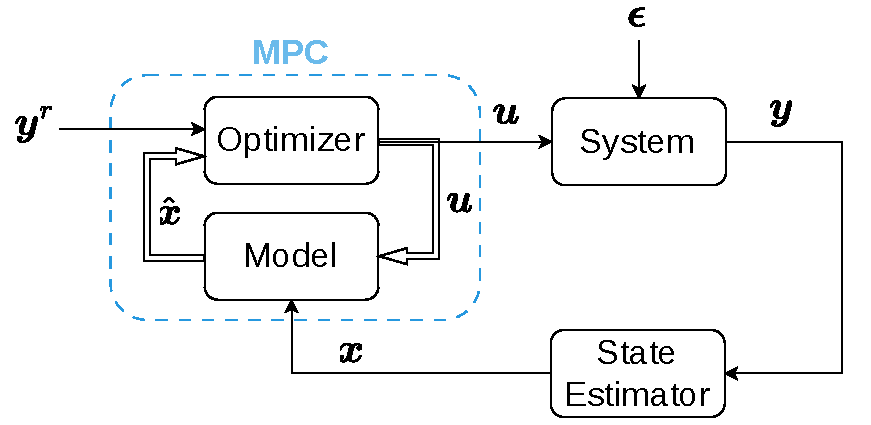
\includegraphics[width=\textwidth]{figures/MPC.pdf} 
        \caption[Schematic of Model Predictive Control]{Schematic of \ac{MPC} for a system with disturbance $\boldsymbol{\epsilon}$. This figure is adapted from \cite{Schwenzer2021}.}
        \label{fig:mpc}
    \end{subfigure}%
    ~ 
    \begin{subfigure}[b]{0.35\textwidth}
        \centering
        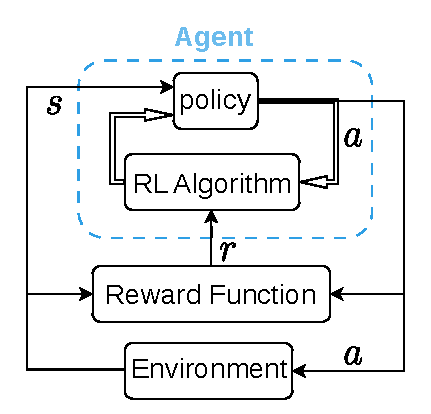
\includegraphics[width=\textwidth]{figures/RL.pdf} 
        \caption[Block diagram of Reinforcement Learning]{Block diagram of \ac{RL}. }
        \label{fig:rl}
    \end{subfigure}
    \caption{\ac{MPC} and \ac{RL}.}
\end{figure*}

After investigating Bayesian system identification and state estimation, we now turn our attention to control strategies, meaning the optimization of system inputs given target and system observations. Control methods can be broadly categorized into model-based and model-free approaches. Model-based control relies on an explicit model of the system dynamics to predict future states and optimize control actions accordingly. In contrast, model-free control approaches do not require a state transition model of the system, instead learning control strategies directly through interactions with the system. A prominent example of model-based control is \acf{MPC} \citep{mpcreview1989, mpcbook2020}. 

\subsubsection{Nominal Model Predictive Control}
A system to be controlled is first modeled in discrete time:
\begin{subequations}
\begin{align}
    \label{eq:mpc_model}
    \boldsymbol{x}_{n+1} &= f(\boldsymbol{x}_n, \boldsymbol{u}_n), \\
    \boldsymbol{y}_n &= h(\boldsymbol{x}_n),
\end{align}
\end{subequations}
where $\boldsymbol{x}_n$ is the system state, $\boldsymbol{u}_n$ and $\boldsymbol{y}_n$ are the control input and system output at time step $n$, respectively. The function $f$ describes the state transition, and $h$ is the measurement function. 

\begin{figure}[htbp]
    \centering
    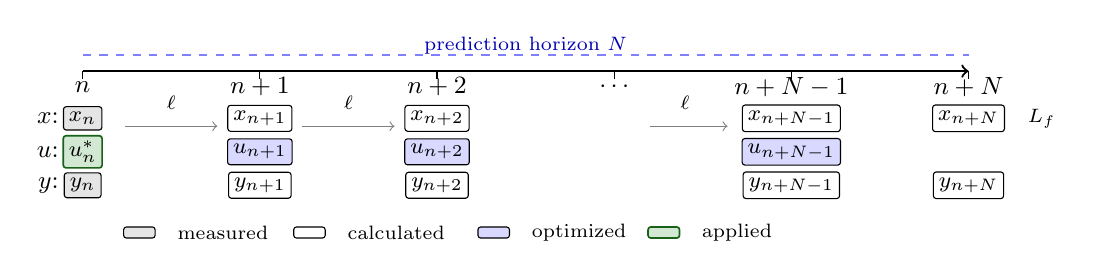
\begin{tikzpicture}[
    time/.style={font=\small},
    var/.style={font=\footnotesize, inner sep=2pt, draw, rounded corners=1pt},
    known/.style={fill=gray!20},
    calc/.style={fill=white},
    opt/.style={fill=blue!15},
    applied/.style={fill=ForestGreen!20, draw=ForestGreen!70!black, line width=0.6pt},
    horizon/.style={dashed, thick, draw=blue!50},
    x=0.9cm, y=0.5cm
]
    % Prediction horizon - above timeline
    \draw[horizon] (0, 2.6) -- (12.5, 2.6);
    \node[font=\scriptsize, blue!70!black] at (6.25, 2.85) {prediction horizon $N$};
    % Timeline
    \draw[->, thick] (0,2.2) -- (12.5,2.2);
    \foreach \x/\lbl in {0/n, 2.5/n+1, 5/n+2, 7.5/\cdots, 10/n+N-1, 12.5/n+N} {
        \draw (\x,2.2) -- (\x,2.0);
        \node[time] at (\x,1.8) {$\lbl$};
    }
    % State row (y=1.0)
    \node[time, anchor=east] at (-0.2, 1.0) {$\boldsymbol{x}$:};
    \node[var, known] at (0, 1.0) {$\boldsymbol{x}_n$};
    \node[var, calc] at (2.5, 1.0) {$\boldsymbol{x}_{n+1}$};
    \node[var, calc] at (5, 1.0) {$\boldsymbol{x}_{n+2}$};
    \node[var, calc] at (10, 1.0) {$\boldsymbol{x}_{n+N-1}$};
    \node[var, calc] at (12.5, 1.0) {$\boldsymbol{x}_{n+N}$};
    % Control row (y=0.15) - more room below x
    \node[time, anchor=east] at (-0.2, 0.15) {$\boldsymbol{u}$:};
    \node[var, applied] at (0, 0.15) {$\boldsymbol{u}_n^*$};
    \node[var, opt] at (2.5, 0.15) {$\boldsymbol{u}_{n+1}$};
    \node[var, opt] at (5, 0.15) {$\boldsymbol{u}_{n+2}$};
    \node[var, opt] at (10, 0.15) {$\boldsymbol{u}_{n+N-1}$};
    % Output row (y=-0.7) - more room below u (u-y gap larger than x-u)
    \node[time, anchor=east] at (-0.2, -0.7) {$\boldsymbol{y}$:};
    \node[var, known] at (0, -0.7) {$\boldsymbol{y}_n$};
    \node[var, calc] at (2.5, -0.7) {$\boldsymbol{y}_{n+1}$};
    \node[var, calc] at (5, -0.7) {$\boldsymbol{y}_{n+2}$};
    \node[var, calc] at (10, -0.7) {$\boldsymbol{y}_{n+N-1}$};
    \node[var, calc] at (12.5, -0.7) {$\boldsymbol{y}_{n+N}$};
    % Cost labels - between timeline and state row
    \node[font=\scriptsize] at (1.25, 1.4) {$\ell$};
    \node[font=\scriptsize] at (3.75, 1.4) {$\ell$};
    \node[font=\scriptsize] at (8.5, 1.4) {$\ell$};
    \node[font=\scriptsize, anchor=west] at (13.2, 1.0) {$L_f$};
    % Dynamics arrows (x_i, u_i) -> x_{i+1}
    \draw[->, gray, thin] (0.6, 0.8) -- (1.9, 0.8);
    \draw[->, gray, thin] (3.1, 0.8) -- (4.4, 0.8);
    \draw[->, gray, thin] (8.0, 0.8) -- (9.1, 0.8);
    % Legend
    \node[var, known, minimum width=0.4cm] at (0.8, -1.9) {};
    \node[font=\scriptsize, anchor=west] at (1.2, -1.9) {measured};
    \node[var, calc, minimum width=0.4cm] at (3.2, -1.9) {};
    \node[font=\scriptsize, anchor=west] at (3.6, -1.9) {calculated};
    \node[var, opt, minimum width=0.4cm] at (5.8, -1.9) {};
    \node[font=\scriptsize, anchor=west] at (6.2, -1.9) {optimized};
    \node[var, applied, minimum width=0.4cm] at (8.2, -1.9) {};
    \node[font=\scriptsize, anchor=west] at (8.6, -1.9) {applied};
\end{tikzpicture}

    \caption[MPC time dependency]{Time dependency of variables in \ac{MPC}. The state $\boldsymbol{x}_n$ is measured at the current step. The optimizer finds $\boldsymbol{u}_{n:n+N-1}$; only $\boldsymbol{u}^*_n$ is applied. Dynamics $f$ and output $h$ propagate along the horizon. Stage costs $\ell$ sum over $i=n,\ldots,n+N-1$; $L_f$ is the terminal cost.}
    \label{fig:mpc_timeline}
\end{figure}

Assuming that a full measurement or estimate of the state $\boldsymbol{x}_n$ is available, the objective of \ac{MPC} is to find an optimal sequence of control inputs $\boldsymbol{u}_{n:n+N-1}$ over a finite prediction horizon $N$. The objective function is:
\begin{subequations}
    \label{eq:mpc}
    \begin{gather}
        \min_{\boldsymbol{u}_{n:n+N-1}} \sum_{i=n}^{n+N-1}\ell(\boldsymbol{y}_{i}, \boldsymbol{u}_{i}, \boldsymbol{y}^r_{i})+L_f(\boldsymbol{y}^r_{n+N},\boldsymbol{y}_{n+N}),\\
        \ell(\boldsymbol{y}_{i}, \boldsymbol{u}_{i}, \boldsymbol{y}^r_{i})=(\boldsymbol{y}_{i}-\boldsymbol{y}^r_{i})^TQ_y(\boldsymbol{y}_{i}-\boldsymbol{y}^r_{i})+\boldsymbol{u}_{i}^TQ_u\boldsymbol{u}_{i},\\
        \text{subject to} \quad \boldsymbol{x}_{i+1} = f(\boldsymbol{x}_i, \boldsymbol{u}_i), \quad \boldsymbol{y}_i = h(\boldsymbol{x}_i),\\
        g_j(\boldsymbol{x}_i, \boldsymbol{u}_i)\leq 0, \quad j=1,\ldots,n_g, \quad i=n,\ldots,n+N-1,\\
        \boldsymbol{u}_{min}\leq\boldsymbol{u}_i\leq\boldsymbol{u}_{max}, \quad i=n,\ldots,n+N-1.
    \end{gather}
\end{subequations}
Figure~\ref{fig:mpc_timeline} illustrates the time dependency of the variables in the \ac{MPC} formulation. At the current time step $n$, the state $\boldsymbol{x}_n$ is measured or estimated. The optimizer computes the control sequence $\boldsymbol{u}_{n:n+N-1}$; only the first element $\boldsymbol{u}^*_n$ is applied to the system. The dynamics $f$ and measurement $h$ propagate states and outputs over the prediction horizon. The stage cost $\ell$ is evaluated at each step $i=n,\ldots,n+N-1$, and the final cost $L_f$ at the terminal step $n+N$.

The cost function consists of a sum of stage costs $\ell$ and a final cost function $L_f$. In the stage cost, weighting matrices $Q_y$ and $Q_u$ are used to balance the trade-off between tracking performance and control effort. The reference trajectory $\boldsymbol{y}^r$ represents the desired output over the prediction horizon. The constraints $g_j(\boldsymbol{x}_i, \boldsymbol{u}_i)\leq 0$ can represent physical limitations of the system or other operational constraints. A simplified schematic of \ac{MPC} is shown in Figure~\ref{fig:mpc}. 

The optimization problem in \ac{MPC} can be solved using various numerical methods, such as sequential quadratic programming, interior-point methods, or gradient-based approaches \citep{Diehl2013}. The choice of method depends on the specific characteristics of the system model and constraints. The first step of the solution (Equation~(\ref{eq:mpc})) $\boldsymbol{u}^*_n$ is applied to the system, and the whole process is repeated at the next time step with updated state information. This is why \ac{MPC} is also known as receding horizon control \citep{Christophersen2007}.

\subsubsection{Stochastic Model Predictive Control}
Taking system uncertainties and disturbances into account, robust \ac{MPC} \citep{rmpc1987} aims to satisfy system stability and constraints despite uncertainties and disturbances. There exist several sound robust \ac{MPC} methods, including Min-Max\ac{MPC} \citep{RAIMONDO20095}, scenario \ac{MPC} \citep{Calafiore_2013}, and stochastic \ac{MPC} \citep{HEIRUNG2018158,smpc2016}. The Min-Max \ac{MPC} chooses control actions that minimize the worst possible cost under bounded disturbances. The scenario \ac{MPC} samples a finite number of random uncertainty realizations as scenarios and optimizes control actions that satisfy constraints for each scenario. Stochastic \ac{MPC} incorporates the probabilistic descriptions of uncertainties into a stochastic optimal control problem through defining chance constraints. A mathematical formulation of stochastic \ac{MPC} is as follows \citep{HEIRUNG2018158} :
\begin{subequations}
    \label{eq:smpc}
    \begin{gather}
        \min_{\boldsymbol{u}_{n:n+N-1}}\sum_{i=n}^{n+N-1}\mathbb{E}[\ell(\boldsymbol{y}_{i}, \boldsymbol{u}_{i}, \boldsymbol{y}^r_{i})]+\mathbb{E}[L_f(\boldsymbol{y}^r_{n+N},\boldsymbol{y}_{n+N})],\\
        \text{subject to} \quad \boldsymbol{x}_{i+1} = f(\boldsymbol{x}_i, \boldsymbol{u}_i, \boldsymbol{w}_i), \quad \boldsymbol{y}_i = h(\boldsymbol{x}_i, \boldsymbol{v}_i),\\
        P[g_j(\boldsymbol{x}_i, \boldsymbol{u}_i)\leq 0]\geq1-\beta_j, \quad\beta_j\in(0,1],\quad j=1,\ldots,n_g, \quad i=n,\ldots,n+N-1,\\
        \boldsymbol{u}_{min}\leq\boldsymbol{u}_i\leq\boldsymbol{u}_{max}, \quad i=n,\ldots,n+N-1.
    \end{gather}    
\end{subequations}   
The chance constraints $P$ regularize the inequality constraints $g_i$, allowing for a small probability $\beta_j$ of constraint violation. The expectation in the cost function can be approximated using Monte Carlo simulation or analytical methods if the distributions are known.                                                                                                                                                                             
\subsection{Reinforcement Learning for Control}
When an accurate model of the system is unavailable or difficult to obtain, model-free control methods can be employed. Classical model-free control methods are \ac{PID} controllers \citep{Fliess_2013}. In recent years, data-driven control methods attract increasing attention. Especially, \acf{RL} can be viewed as a model-free framework for solving optimal control problems, and has been successfully applied in various domains, including robotics, game playing, and autonomous systems.

We first introduce the terminology of \ac{RL}:
\begin{itemize}
\item agent: the controller,
\item environment: the to-be-controlled system,
\item action: the control input, $a_t$,
\item state: the complete state of the environment, $s_t$,
\item policy: the control strategy, which can be deterministic ($a_t=\mu(s_t)$) or probabilistic ($a_t \sim \pi(\cdot|s_t)$),
\item reward: the feedback on the agent's success, $r_t=R(s_t,a_t)$.
\end{itemize}
The foundation of \ac{RL} is the \ac{MDP} \citep{mdp2014}. An \ac{MDP} is defined by the tuple $(\mathcal{S}, \mathcal{A}, P, R, \gamma)$, where $\mathcal{S}$ is the set of states, $\mathcal{A}$ is the set of actions, $P(s_{t+1}|s_t,a_t)$ is the state transition probability, $R(s_t,a_t)$ is the reward function, and $\gamma\in[0,1]$ is the discount factor. The interaction process between the agent and the environment at each time step $t$ is as follows: the agent observes the current state $s_t$, selects an action $a_t$ according to its policy $\pi(a_t|s_t)$, receives a reward $r_t=R(s_t,a_t)$ from the environment, and transitions to a new state $s_{t+1}$ based on the state transition probability $P(s_{t+1}|s_t,a_t)$. The goal of the agent is to learn an optimal policy $\pi^*$ that maximizes the expected return, i.e., the value function:
\begin{equation}
    \pi^* = \arg\max_{\pi} \mathbb{E}_{\pi}\left[\sum_{t=0}^{\infty} \gamma^t r_t\right].
\end{equation}          

In comparison to other optimal control methods, \ac{RL} methods aim to optimize long-term sequential decision-making performance. Besides, generality and scalability are the two main advantages of \ac{RL} methods. They can handle nonlinear, high-dimensional, and stochastic dynamics and also non-quadratic reward functions. The work by \citeauthor{rlforcontrol2018} \citeyearpar{rlforcontrol2018} provides a comprehensive review of \ac{RL} for control. 

It is worth noting that there is also an \ac{RL} method applying a surrogate model for the sake of improving the policy, which is called model-based \ac{RL} \citep{sutton1990, mbrl2020}. The surrogate model is learned from data in advance. Then, the model can also be used for planning, simulation, or generating synthetic data to augment real-world data. In comparison to the model-free \ac{RL}, the model-based \ac{RL} can reduce the required amount of samples gathered directly from the environment. From the viewpoint of control, model-based \ac{RL} is also referred to learning-based control, when the surrogate model is also adaptive online. From the perspective of leveraging a state transition model, model-based \ac{RL} can be viewed as a hybrid approach that combines elements of both model-based and model-free control strategies.

\ac{RL} provides a flexible framework for learning control policies directly from data, enabling adaptation to changing environments and complex system dynamics. However, it often requires a large amount of data and may suffer from explainability, stability, and reliability issues. In safety-critical applications, model-based control methods are often preferred.